\documentclass[1p]{elsarticle_modified}
%\bibliographystyle{elsarticle-num}

%\usepackage[colorlinks]{hyperref}
%\usepackage{abbrmath_seonhwa} %\Abb, \Ascr, \Acal ,\Abf, \Afrak
\usepackage{amsfonts}
\usepackage{amssymb}
\usepackage{amsmath}
\usepackage{amsthm}
\usepackage{scalefnt}
\usepackage{amsbsy}
\usepackage{kotex}
\usepackage{caption}
\usepackage{subfig}
\usepackage{color}
\usepackage{graphicx}
\usepackage{xcolor} %% white, black, red, green, blue, cyan, magenta, yellow
\usepackage{float}
\usepackage{setspace}
\usepackage{hyperref}

\usepackage{tikz}
\usetikzlibrary{arrows}

\usepackage{multirow}
\usepackage{array} % fixed length table
\usepackage{hhline}

%%%%%%%%%%%%%%%%%%%%%
\makeatletter
\renewcommand*\env@matrix[1][\arraystretch]{%
	\edef\arraystretch{#1}%
	\hskip -\arraycolsep
	\let\@ifnextchar\new@ifnextchar
	\array{*\c@MaxMatrixCols c}}
\makeatother %https://tex.stackexchange.com/questions/14071/how-can-i-increase-the-line-spacing-in-a-matrix
%%%%%%%%%%%%%%%

\usepackage[normalem]{ulem}

\newcommand{\msout}[1]{\ifmmode\text{\sout{\ensuremath{#1}}}\else\sout{#1}\fi}
%SOURCE: \msout is \stkout macro in https://tex.stackexchange.com/questions/20609/strikeout-in-math-mode

\newcommand{\cancel}[1]{
	\ifmmode
	{\color{red}\msout{#1}}
	\else
	{\color{red}\sout{#1}}
	\fi
}

\newcommand{\add}[1]{
	{\color{blue}\uwave{#1}}
}

\newcommand{\replace}[2]{
	\ifmmode
	{\color{red}\msout{#1}}{\color{blue}\uwave{#2}}
	\else
	{\color{red}\sout{#1}}{\color{blue}\uwave{#2}}
	\fi
}

\newcommand{\Sol}{\mathcal{S}} %segment
\newcommand{\D}{D} %diagram
\newcommand{\A}{\mathcal{A}} %arc


%%%%%%%%%%%%%%%%%%%%%%%%%%%%%5 test

\def\sl{\operatorname{\textup{SL}}(2,\Cbb)}
\def\psl{\operatorname{\textup{PSL}}(2,\Cbb)}
\def\quan{\mkern 1mu \triangleright \mkern 1mu}

\theoremstyle{definition}
\newtheorem{thm}{Theorem}[section]
\newtheorem{prop}[thm]{Proposition}
\newtheorem{lem}[thm]{Lemma}
\newtheorem{ques}[thm]{Question}
\newtheorem{cor}[thm]{Corollary}
\newtheorem{defn}[thm]{Definition}
\newtheorem{exam}[thm]{Example}
\newtheorem{rmk}[thm]{Remark}
\newtheorem{alg}[thm]{Algorithm}

\newcommand{\I}{\sqrt{-1}}
\begin{document}

%\begin{frontmatter}
%
%\title{Boundary parabolic representations of knots up to 8 crossings}
%
%%% Group authors per affiliation:
%\author{Yunhi Cho} 
%\address{Department of Mathematics, University of Seoul, Seoul, Korea}
%\ead{yhcho@uos.ac.kr}
%
%
%\author{Seonhwa Kim} %\fnref{s_kim}}
%\address{Center for Geometry and Physics, Institute for Basic Science, Pohang, 37673, Korea}
%\ead{ryeona17@ibs.re.kr}
%
%\author{Hyuk Kim}
%\address{Department of Mathematical Sciences, Seoul National University, Seoul 08826, Korea}
%\ead{hyukkim@snu.ac.kr}
%
%\author{Seokbeom Yoon}
%\address{Department of Mathematical Sciences, Seoul National University, Seoul, 08826,  Korea}
%\ead{sbyoon15@snu.ac.kr}
%
%\begin{abstract}
%We find all boundary parabolic representation of knots up to 8 crossings.
%
%\end{abstract}
%\begin{keyword}
%    \MSC[2010] 57M25 
%\end{keyword}
%
%\end{frontmatter}

%\linenumbers
%\tableofcontents
%
\newcommand\colored[1]{\textcolor{white}{\rule[-0.35ex]{0.8em}{1.4ex}}\kern-0.8em\color{red} #1}%
%\newcommand\colored[1]{\textcolor{white}{ #1}\kern-2.17ex	\textcolor{white}{ #1}\kern-1.81ex	\textcolor{white}{ #1}\kern-2.15ex\color{red}#1	}

{\Large $\underline{12a_{0998}~(K12a_{0998})}$}

\setlength{\tabcolsep}{10pt}
\renewcommand{\arraystretch}{1.6}
\vspace{1cm}\begin{tabular}{m{100pt}>{\centering\arraybackslash}m{274pt}}
\multirow{5}{120pt}{
	\centering
	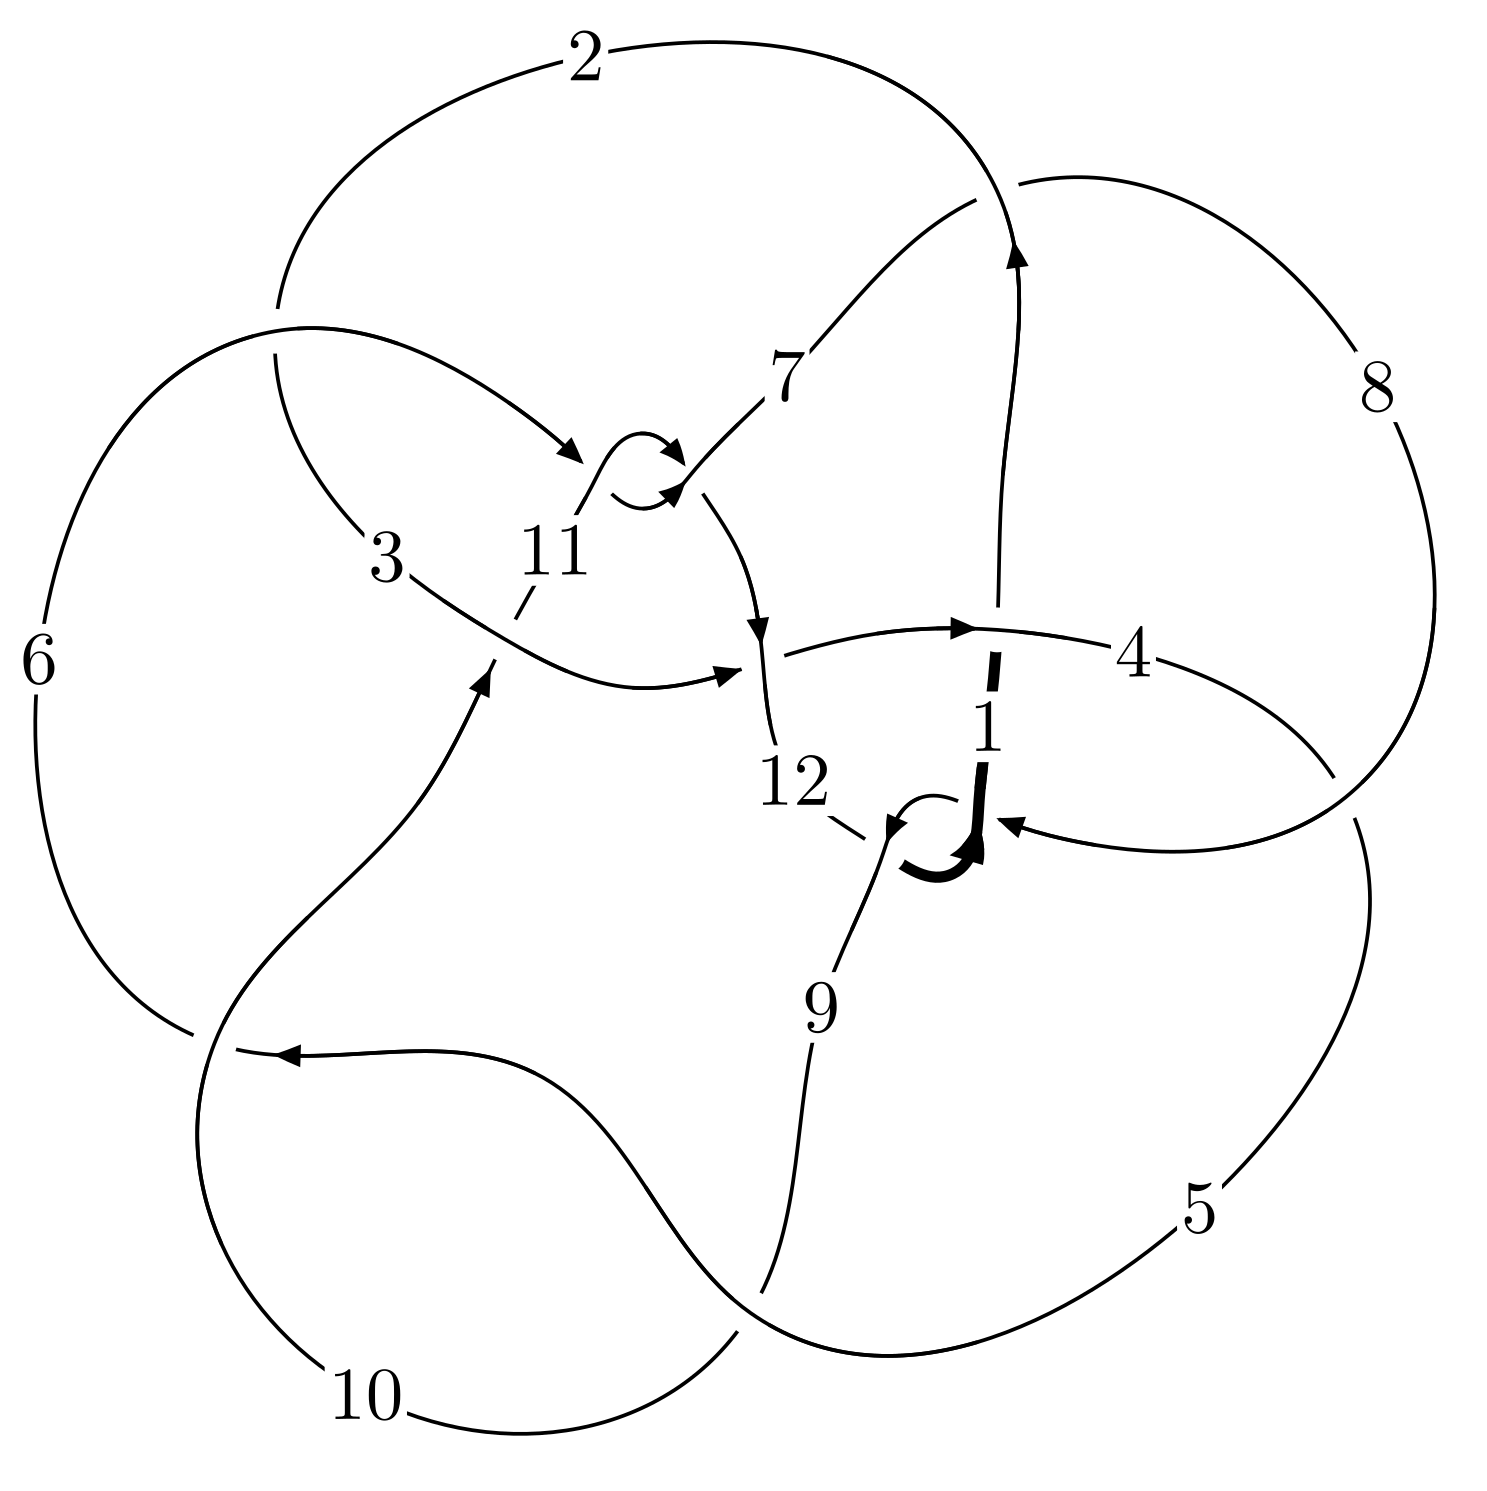
\includegraphics[width=112pt]{../../../GIT/diagram.site/Diagrams/png/1799_12a_0998.png}\\
\ \ \ A knot diagram\footnotemark}&
\allowdisplaybreaks
\textbf{Linearized knot diagam} \\
\cline{2-2}
 &
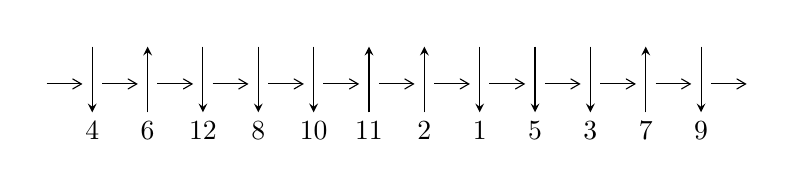
\begin{tikzpicture}[x=20pt, y=17pt]
	% nodes
	\node (C0) at (0, 0) {};
	\node (C1) at (1, 0) {};
	\node (C1U) at (1, +1) {};
	\node (C1D) at (1, -1) {4};

	\node (C2) at (2, 0) {};
	\node (C2U) at (2, +1) {};
	\node (C2D) at (2, -1) {6};

	\node (C3) at (3, 0) {};
	\node (C3U) at (3, +1) {};
	\node (C3D) at (3, -1) {12};

	\node (C4) at (4, 0) {};
	\node (C4U) at (4, +1) {};
	\node (C4D) at (4, -1) {8};

	\node (C5) at (5, 0) {};
	\node (C5U) at (5, +1) {};
	\node (C5D) at (5, -1) {10};

	\node (C6) at (6, 0) {};
	\node (C6U) at (6, +1) {};
	\node (C6D) at (6, -1) {11};

	\node (C7) at (7, 0) {};
	\node (C7U) at (7, +1) {};
	\node (C7D) at (7, -1) {2};

	\node (C8) at (8, 0) {};
	\node (C8U) at (8, +1) {};
	\node (C8D) at (8, -1) {1};

	\node (C9) at (9, 0) {};
	\node (C9U) at (9, +1) {};
	\node (C9D) at (9, -1) {5};

	\node (C10) at (10, 0) {};
	\node (C10U) at (10, +1) {};
	\node (C10D) at (10, -1) {3};

	\node (C11) at (11, 0) {};
	\node (C11U) at (11, +1) {};
	\node (C11D) at (11, -1) {7};

	\node (C12) at (12, 0) {};
	\node (C12U) at (12, +1) {};
	\node (C12D) at (12, -1) {9};
	\node (C13) at (13, 0) {};

	% arrows
	\draw[->,>={angle 60}]
	(C0) edge (C1) (C1) edge (C2) (C2) edge (C3) (C3) edge (C4) (C4) edge (C5) (C5) edge (C6) (C6) edge (C7) (C7) edge (C8) (C8) edge (C9) (C9) edge (C10) (C10) edge (C11) (C11) edge (C12) (C12) edge (C13) ;	\draw[->,>=stealth]
	(C1U) edge (C1D) (C2D) edge (C2U) (C3U) edge (C3D) (C4U) edge (C4D) (C5U) edge (C5D) (C6D) edge (C6U) (C7D) edge (C7U) (C8U) edge (C8D) (C9U) edge (C9D) (C10U) edge (C10D) (C11D) edge (C11U) (C12U) edge (C12D) ;
	\end{tikzpicture} \\
\hhline{~~} \\& 
\textbf{Solving Sequence} \\ \cline{2-2} 
 &
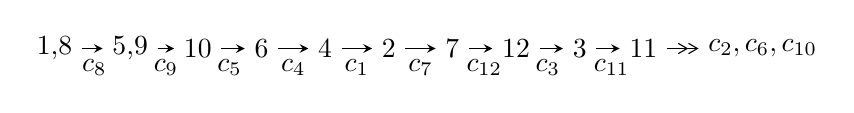
\begin{tikzpicture}[x=23pt, y=7pt]
	% node
	\node (A0) at (-1/8, 0) {1,8};
	\node (A1) at (17/16, 0) {5,9};
	\node (A2) at (17/8, 0) {10};
	\node (A3) at (25/8, 0) {6};
	\node (A4) at (33/8, 0) {4};
	\node (A5) at (41/8, 0) {2};
	\node (A6) at (49/8, 0) {7};
	\node (A7) at (57/8, 0) {12};
	\node (A8) at (65/8, 0) {3};
	\node (A9) at (73/8, 0) {11};
	\node (C1) at (1/2, -1) {$c_{8}$};
	\node (C2) at (13/8, -1) {$c_{9}$};
	\node (C3) at (21/8, -1) {$c_{5}$};
	\node (C4) at (29/8, -1) {$c_{4}$};
	\node (C5) at (37/8, -1) {$c_{1}$};
	\node (C6) at (45/8, -1) {$c_{7}$};
	\node (C7) at (53/8, -1) {$c_{12}$};
	\node (C8) at (61/8, -1) {$c_{3}$};
	\node (C9) at (69/8, -1) {$c_{11}$};
	\node (A10) at (11, 0) {$c_{2},c_{6},c_{10}$};

	% edge
	\draw[->,>=stealth]	
	(A0) edge (A1) (A1) edge (A2) (A2) edge (A3) (A3) edge (A4) (A4) edge (A5) (A5) edge (A6) (A6) edge (A7) (A7) edge (A8) (A8) edge (A9) ;
	\draw[->>,>={angle 60}]	
	(A9) edge (A10);
\end{tikzpicture} \\ 

\end{tabular} \\

\footnotetext{
The image of knot diagram is generated by the software ``\textbf{Draw programme}" developed by Andrew Bartholomew(\url{http://www.layer8.co.uk/maths/draw/index.htm\#Running-draw}), where we modified some parts for our purpose(\url{https://github.com/CATsTAILs/LinksPainter}).
}\phantom \\ \newline 
\centering \textbf{Ideals for irreducible components\footnotemark of $X_{\text{par}}$} 
 
\begin{align*}
I^u_{1}&=\langle 
9.23532\times10^{824} u^{161}-6.57296\times10^{825} u^{160}+\cdots+3.97408\times10^{825} b+3.77915\times10^{828},\\
\phantom{I^u_{1}}&\phantom{= \langle  }8.54087\times10^{826} u^{161}+2.27504\times10^{828} u^{160}+\cdots+5.48026\times10^{828} a-3.72721\times10^{831},\\
\phantom{I^u_{1}}&\phantom{= \langle  }u^{162}-5 u^{161}+\cdots+9133 u-1379\rangle \\
I^u_{2}&=\langle 
1.78669\times10^{27} u^{36}+1.25651\times10^{26} u^{35}+\cdots+2.72369\times10^{26} b+1.59434\times10^{27},\\
\phantom{I^u_{2}}&\phantom{= \langle  }-4.27607\times10^{26} u^{36}-2.28243\times10^{26} u^{35}+\cdots+9.07896\times10^{25} a-8.22612\times10^{26},\\
\phantom{I^u_{2}}&\phantom{= \langle  }u^{37}+13 u^{35}+\cdots+4 u+1\rangle \\
\\
\end{align*}
\raggedright * 2 irreducible components of $\dim_{\mathbb{C}}=0$, with total 199 representations.\\
\footnotetext{All coefficients of polynomials are rational numbers. But the coefficients are sometimes approximated in decimal forms when there is not enough margin.}
\newpage
\renewcommand{\arraystretch}{1}
\centering \section*{I. $I^u_{1}= \langle 9.24\times10^{824} u^{161}-6.57\times10^{825} u^{160}+\cdots+3.97\times10^{825} b+3.78\times10^{828},\;8.54\times10^{826} u^{161}+2.28\times10^{828} u^{160}+\cdots+5.48\times10^{828} a-3.73\times10^{831},\;u^{162}-5 u^{161}+\cdots+9133 u-1379 \rangle$}
\flushleft \textbf{(i) Arc colorings}\\
\begin{tabular}{m{7pt} m{180pt} m{7pt} m{180pt} }
\flushright $a_{1}=$&$\begin{pmatrix}0\\u\end{pmatrix}$ \\
\flushright $a_{8}=$&$\begin{pmatrix}1\\0\end{pmatrix}$ \\
\flushright $a_{5}=$&$\begin{pmatrix}-0.0155848 u^{161}-0.415133 u^{160}+\cdots-4034.89 u+680.116\\-0.232389 u^{161}+1.65396 u^{160}+\cdots+6136.17 u-950.950\end{pmatrix}$ \\
\flushright $a_{9}=$&$\begin{pmatrix}1\\u^2\end{pmatrix}$ \\
\flushright $a_{10}=$&$\begin{pmatrix}0.249366 u^{161}-0.732722 u^{160}+\cdots+3590.36 u-671.653\\0.135745 u^{161}-1.05334 u^{160}+\cdots-4779.66 u+770.743\end{pmatrix}$ \\
\flushright $a_{6}=$&$\begin{pmatrix}-0.0466441 u^{161}+0.613048 u^{160}+\cdots+5373.45 u-850.883\\0.350662 u^{161}-1.95858 u^{160}+\cdots-4358.67 u+625.210\end{pmatrix}$ \\
\flushright $a_{4}=$&$\begin{pmatrix}-0.247974 u^{161}+1.23882 u^{160}+\cdots+2101.28 u-270.834\\-0.232389 u^{161}+1.65396 u^{160}+\cdots+6136.17 u-950.950\end{pmatrix}$ \\
\flushright $a_{2}=$&$\begin{pmatrix}0.00569413 u^{161}+0.433509 u^{160}+\cdots+4147.58 u-695.597\\0.152721 u^{161}-0.692554 u^{160}+\cdots-352.971 u+8.02221\end{pmatrix}$ \\
\flushright $a_{7}=$&$\begin{pmatrix}-0.998800 u^{161}+4.54500 u^{160}+\cdots+1553.00 u+63.4474\\-0.398050 u^{161}+2.01079 u^{160}+\cdots+2899.90 u-364.505\end{pmatrix}$ \\
\flushright $a_{12}=$&$\begin{pmatrix}u\\u^3+u\end{pmatrix}$ \\
\flushright $a_{3}=$&$\begin{pmatrix}0.0423463 u^{161}-0.419826 u^{160}+\cdots-1724.26 u+272.260\\-0.244538 u^{161}+1.52800 u^{160}+\cdots+4601.97 u-693.378\end{pmatrix}$ \\
\flushright $a_{11}=$&$\begin{pmatrix}0.813964 u^{161}-3.50192 u^{160}+\cdots+875.215 u-366.609\\0.153738 u^{161}-0.776005 u^{160}+\cdots-978.802 u+117.885\end{pmatrix}$\\&\end{tabular}
\flushleft \textbf{(ii) Obstruction class $= -1$}\\~\\
\flushleft \textbf{(iii) Cusp Shapes $= -0.322129 u^{161}+0.340512 u^{160}+\cdots-12922.8 u+2312.72$}\\~\\
\newpage\renewcommand{\arraystretch}{1}
\flushleft \textbf{(iv) u-Polynomials at the component}\newline \\
\begin{tabular}{m{50pt}|m{274pt}}
Crossings & \hspace{64pt}u-Polynomials at each crossing \\
\hline $$\begin{aligned}c_{1}\end{aligned}$$&$\begin{aligned}
&u^{162}+10 u^{161}+\cdots+154 u-7
\end{aligned}$\\
\hline $$\begin{aligned}c_{2}\end{aligned}$$&$\begin{aligned}
&u^{162}+8 u^{160}+\cdots-20 u+1
\end{aligned}$\\
\hline $$\begin{aligned}c_{3}\end{aligned}$$&$\begin{aligned}
&u^{162}-2 u^{161}+\cdots+7626293679 u+965121761
\end{aligned}$\\
\hline $$\begin{aligned}c_{4}\end{aligned}$$&$\begin{aligned}
&u^{162}+7 u^{161}+\cdots+31 u-1
\end{aligned}$\\
\hline $$\begin{aligned}c_{5},c_{9}\end{aligned}$$&$\begin{aligned}
&u^{162}-3 u^{161}+\cdots+6218386 u-528361
\end{aligned}$\\
\hline $$\begin{aligned}c_{6},c_{11}\end{aligned}$$&$\begin{aligned}
&u^{162}-51 u^{160}+\cdots+1717 u+437
\end{aligned}$\\
\hline $$\begin{aligned}c_{7}\end{aligned}$$&$\begin{aligned}
&u^{162}+u^{161}+\cdots-6589604478 u-630454121
\end{aligned}$\\
\hline $$\begin{aligned}c_{8},c_{12}\end{aligned}$$&$\begin{aligned}
&u^{162}+5 u^{161}+\cdots-9133 u-1379
\end{aligned}$\\
\hline $$\begin{aligned}c_{10}\end{aligned}$$&$\begin{aligned}
&u^{162}-2 u^{161}+\cdots+123 u-7
\end{aligned}$\\
\hline
\end{tabular}\\~\\
\newpage\renewcommand{\arraystretch}{1}
\flushleft \textbf{(v) Riley Polynomials at the component}\newline \\
\begin{tabular}{m{50pt}|m{274pt}}
Crossings & \hspace{64pt}Riley Polynomials at each crossing \\
\hline $$\begin{aligned}c_{1}\end{aligned}$$&$\begin{aligned}
&y^{162}+4 y^{161}+\cdots-4116 y+49
\end{aligned}$\\
\hline $$\begin{aligned}c_{2}\end{aligned}$$&$\begin{aligned}
&y^{162}+16 y^{161}+\cdots-190 y+1
\end{aligned}$\\
\hline $$\begin{aligned}c_{3}\end{aligned}$$&$\begin{aligned}
&y^{162}-54 y^{161}+\cdots-2.99\times10^{18} y+9.31\times10^{17}
\end{aligned}$\\
\hline $$\begin{aligned}c_{4}\end{aligned}$$&$\begin{aligned}
&y^{162}-13 y^{161}+\cdots-17 y+1
\end{aligned}$\\
\hline $$\begin{aligned}c_{5},c_{9}\end{aligned}$$&$\begin{aligned}
&y^{162}-131 y^{161}+\cdots-29177786074 y+279165346321
\end{aligned}$\\
\hline $$\begin{aligned}c_{6},c_{11}\end{aligned}$$&$\begin{aligned}
&y^{162}-102 y^{161}+\cdots-3102787 y+190969
\end{aligned}$\\
\hline $$\begin{aligned}c_{7}\end{aligned}$$&$\begin{aligned}
&y^{162}+73 y^{161}+\cdots+2.01\times10^{19} y+3.97\times10^{17}
\end{aligned}$\\
\hline $$\begin{aligned}c_{8},c_{12}\end{aligned}$$&$\begin{aligned}
&y^{162}+97 y^{161}+\cdots-11736785 y+1901641
\end{aligned}$\\
\hline $$\begin{aligned}c_{10}\end{aligned}$$&$\begin{aligned}
&y^{162}-6 y^{161}+\cdots-5063 y+49
\end{aligned}$\\
\hline
\end{tabular}\\~\\
\newpage\flushleft \textbf{(vi) Complex Volumes and Cusp Shapes}
$$\begin{array}{c|c|c}  
\text{Solutions to }I^u_{1}& \I (\text{vol} + \sqrt{-1}CS) & \text{Cusp shape}\\
 \hline 
\begin{aligned}
u &= -0.364438 + 0.934578 I \\
a &= \phantom{-}0.86922 - 1.96405 I \\
b &= -0.332857 + 0.194362 I\end{aligned}
 & -5.55873 + 5.66135 I & \phantom{-0.000000 } 0 \\ \hline\begin{aligned}
u &= -0.364438 - 0.934578 I \\
a &= \phantom{-}0.86922 + 1.96405 I \\
b &= -0.332857 - 0.194362 I\end{aligned}
 & -5.55873 - 5.66135 I & \phantom{-0.000000 } 0 \\ \hline\begin{aligned}
u &= -0.072129 + 1.027860 I \\
a &= -0.636429 - 0.480890 I \\
b &= -0.172441 + 0.679991 I\end{aligned}
 & \phantom{-}2.29357 - 2.45523 I & \phantom{-0.000000 } 0 \\ \hline\begin{aligned}
u &= -0.072129 - 1.027860 I \\
a &= -0.636429 + 0.480890 I \\
b &= -0.172441 - 0.679991 I\end{aligned}
 & \phantom{-}2.29357 + 2.45523 I & \phantom{-0.000000 } 0 \\ \hline\begin{aligned}
u &= \phantom{-}0.470589 + 0.920034 I \\
a &= -0.07190 - 2.12268 I \\
b &= \phantom{-}0.76812 + 1.60658 I\end{aligned}
 & -0.83623 - 4.97202 I & \phantom{-0.000000 } 0 \\ \hline\begin{aligned}
u &= \phantom{-}0.470589 - 0.920034 I \\
a &= -0.07190 + 2.12268 I \\
b &= \phantom{-}0.76812 - 1.60658 I\end{aligned}
 & -0.83623 + 4.97202 I & \phantom{-0.000000 } 0 \\ \hline\begin{aligned}
u &= \phantom{-}0.220408 + 1.010250 I \\
a &= -0.400546 - 1.323730 I \\
b &= -0.315050 + 1.042240 I\end{aligned}
 & \phantom{-}1.89460 - 2.94833 I & \phantom{-0.000000 } 0 \\ \hline\begin{aligned}
u &= \phantom{-}0.220408 - 1.010250 I \\
a &= -0.400546 + 1.323730 I \\
b &= -0.315050 - 1.042240 I\end{aligned}
 & \phantom{-}1.89460 + 2.94833 I & \phantom{-0.000000 } 0 \\ \hline\begin{aligned}
u &= \phantom{-}0.450212 + 0.931702 I \\
a &= -0.54552 - 1.99644 I \\
b &= \phantom{-}0.543613 + 0.211021 I\end{aligned}
 & -2.71791 - 11.48510 I & \phantom{-0.000000 } 0 \\ \hline\begin{aligned}
u &= \phantom{-}0.450212 - 0.931702 I \\
a &= -0.54552 + 1.99644 I \\
b &= \phantom{-}0.543613 - 0.211021 I\end{aligned}
 & -2.71791 + 11.48510 I & \phantom{-0.000000 } 0\\
 \hline 
 \end{array}$$\newpage$$\begin{array}{c|c|c}  
\text{Solutions to }I^u_{1}& \I (\text{vol} + \sqrt{-1}CS) & \text{Cusp shape}\\
 \hline 
\begin{aligned}
u &= -0.824197 + 0.640695 I \\
a &= \phantom{-}0.172573 - 0.338696 I \\
b &= \phantom{-}1.034890 - 0.230430 I\end{aligned}
 & -3.03988 + 5.26417 I & \phantom{-0.000000 } 0 \\ \hline\begin{aligned}
u &= -0.824197 - 0.640695 I \\
a &= \phantom{-}0.172573 + 0.338696 I \\
b &= \phantom{-}1.034890 + 0.230430 I\end{aligned}
 & -3.03988 - 5.26417 I & \phantom{-0.000000 } 0 \\ \hline\begin{aligned}
u &= \phantom{-}0.372414 + 0.877222 I \\
a &= \phantom{-}1.16096 + 1.73885 I \\
b &= -0.756263 - 0.088084 I\end{aligned}
 & -2.88184 + 0.92994 I & \phantom{-0.000000 } 0 \\ \hline\begin{aligned}
u &= \phantom{-}0.372414 - 0.877222 I \\
a &= \phantom{-}1.16096 - 1.73885 I \\
b &= -0.756263 + 0.088084 I\end{aligned}
 & -2.88184 - 0.92994 I & \phantom{-0.000000 } 0 \\ \hline\begin{aligned}
u &= -0.311668 + 0.895614 I \\
a &= -0.44991 + 2.51594 I \\
b &= \phantom{-}0.511881 - 1.204870 I\end{aligned}
 & -3.42601 + 1.93989 I & \phantom{-0.000000 } 0 \\ \hline\begin{aligned}
u &= -0.311668 - 0.895614 I \\
a &= -0.44991 - 2.51594 I \\
b &= \phantom{-}0.511881 + 1.204870 I\end{aligned}
 & -3.42601 - 1.93989 I & \phantom{-0.000000 } 0 \\ \hline\begin{aligned}
u &= \phantom{-}0.214606 + 0.921083 I \\
a &= -1.86429 + 1.76707 I \\
b &= \phantom{-}2.18602 - 1.91828 I\end{aligned}
 & -1.34785 - 9.76566 I & \phantom{-0.000000 } 0 \\ \hline\begin{aligned}
u &= \phantom{-}0.214606 - 0.921083 I \\
a &= -1.86429 - 1.76707 I \\
b &= \phantom{-}2.18602 + 1.91828 I\end{aligned}
 & -1.34785 + 9.76566 I & \phantom{-0.000000 } 0 \\ \hline\begin{aligned}
u &= \phantom{-}0.363781 + 0.994655 I \\
a &= -0.595660 - 0.023343 I \\
b &= \phantom{-}0.831366 - 0.015985 I\end{aligned}
 & -0.62485 - 1.65369 I & \phantom{-0.000000 } 0 \\ \hline\begin{aligned}
u &= \phantom{-}0.363781 - 0.994655 I \\
a &= -0.595660 + 0.023343 I \\
b &= \phantom{-}0.831366 + 0.015985 I\end{aligned}
 & -0.62485 + 1.65369 I & \phantom{-0.000000 } 0\\
 \hline 
 \end{array}$$\newpage$$\begin{array}{c|c|c}  
\text{Solutions to }I^u_{1}& \I (\text{vol} + \sqrt{-1}CS) & \text{Cusp shape}\\
 \hline 
\begin{aligned}
u &= -0.310080 + 0.888024 I \\
a &= \phantom{-}0.36728 - 2.88425 I \\
b &= -0.65828 + 2.02432 I\end{aligned}
 & -5.38995 - 1.50217 I & \phantom{-0.000000 } 0 \\ \hline\begin{aligned}
u &= -0.310080 - 0.888024 I \\
a &= \phantom{-}0.36728 + 2.88425 I \\
b &= -0.65828 - 2.02432 I\end{aligned}
 & -5.38995 + 1.50217 I & \phantom{-0.000000 } 0 \\ \hline\begin{aligned}
u &= -0.391447 + 0.847504 I \\
a &= -0.66560 + 2.24197 I \\
b &= \phantom{-}0.713508 - 0.549552 I\end{aligned}
 & -3.89774 + 1.76552 I & \phantom{-0.000000 } 0 \\ \hline\begin{aligned}
u &= -0.391447 - 0.847504 I \\
a &= -0.66560 - 2.24197 I \\
b &= \phantom{-}0.713508 + 0.549552 I\end{aligned}
 & -3.89774 - 1.76552 I & \phantom{-0.000000 } 0 \\ \hline\begin{aligned}
u &= -0.912869 + 0.183465 I \\
a &= -0.0037704 + 0.1269540 I \\
b &= -0.284123 + 0.658858 I\end{aligned}
 & \phantom{-}3.84065 - 1.36973 I & \phantom{-0.000000 } 0 \\ \hline\begin{aligned}
u &= -0.912869 - 0.183465 I \\
a &= -0.0037704 - 0.1269540 I \\
b &= -0.284123 - 0.658858 I\end{aligned}
 & \phantom{-}3.84065 + 1.36973 I & \phantom{-0.000000 } 0 \\ \hline\begin{aligned}
u &= -0.970833 + 0.477295 I \\
a &= -0.693410 + 0.238527 I \\
b &= \phantom{-}0.997093 + 0.943625 I\end{aligned}
 & -3.86036 - 4.39205 I & \phantom{-0.000000 } 0 \\ \hline\begin{aligned}
u &= -0.970833 - 0.477295 I \\
a &= -0.693410 - 0.238527 I \\
b &= \phantom{-}0.997093 - 0.943625 I\end{aligned}
 & -3.86036 + 4.39205 I & \phantom{-0.000000 } 0 \\ \hline\begin{aligned}
u &= -0.393745 + 1.010210 I \\
a &= \phantom{-}0.42093 + 1.42013 I \\
b &= \phantom{-}0.963756 - 0.962346 I\end{aligned}
 & \phantom{-}0.77778 + 4.28953 I & \phantom{-0.000000 } 0 \\ \hline\begin{aligned}
u &= -0.393745 - 1.010210 I \\
a &= \phantom{-}0.42093 - 1.42013 I \\
b &= \phantom{-}0.963756 + 0.962346 I\end{aligned}
 & \phantom{-}0.77778 - 4.28953 I & \phantom{-0.000000 } 0\\
 \hline 
 \end{array}$$\newpage$$\begin{array}{c|c|c}  
\text{Solutions to }I^u_{1}& \I (\text{vol} + \sqrt{-1}CS) & \text{Cusp shape}\\
 \hline 
\begin{aligned}
u &= -0.320600 + 1.041220 I \\
a &= -0.67910 - 1.50315 I \\
b &= -0.711051 + 0.543143 I\end{aligned}
 & \phantom{-}3.13808 - 1.44812 I & \phantom{-0.000000 } 0 \\ \hline\begin{aligned}
u &= -0.320600 - 1.041220 I \\
a &= -0.67910 + 1.50315 I \\
b &= -0.711051 - 0.543143 I\end{aligned}
 & \phantom{-}3.13808 + 1.44812 I & \phantom{-0.000000 } 0 \\ \hline\begin{aligned}
u &= -0.116410 + 0.898199 I \\
a &= \phantom{-}0.29642 + 2.39237 I \\
b &= \phantom{-}0.578282 - 1.155400 I\end{aligned}
 & \phantom{-}0.46297 + 3.03319 I & \phantom{-0.000000 } 0 \\ \hline\begin{aligned}
u &= -0.116410 - 0.898199 I \\
a &= \phantom{-}0.29642 - 2.39237 I \\
b &= \phantom{-}0.578282 + 1.155400 I\end{aligned}
 & \phantom{-}0.46297 - 3.03319 I & \phantom{-0.000000 } 0 \\ \hline\begin{aligned}
u &= \phantom{-}0.097092 + 0.897734 I \\
a &= \phantom{-}0.27466 + 2.05124 I \\
b &= \phantom{-}0.88611 - 1.15198 I\end{aligned}
 & \phantom{-}1.19045 + 1.64565 I & \phantom{-0.000000 } 0 \\ \hline\begin{aligned}
u &= \phantom{-}0.097092 - 0.897734 I \\
a &= \phantom{-}0.27466 - 2.05124 I \\
b &= \phantom{-}0.88611 + 1.15198 I\end{aligned}
 & \phantom{-}1.19045 - 1.64565 I & \phantom{-0.000000 } 0 \\ \hline\begin{aligned}
u &= -0.891860 + 0.064694 I \\
a &= -0.428218 - 0.116662 I \\
b &= -0.678883 + 0.845513 I\end{aligned}
 & \phantom{-}0.89156 + 9.33028 I & \phantom{-0.000000 } 0 \\ \hline\begin{aligned}
u &= -0.891860 - 0.064694 I \\
a &= -0.428218 + 0.116662 I \\
b &= -0.678883 - 0.845513 I\end{aligned}
 & \phantom{-}0.89156 - 9.33028 I & \phantom{-0.000000 } 0 \\ \hline\begin{aligned}
u &= \phantom{-}0.786309 + 0.411248 I \\
a &= -0.049283 + 0.540545 I \\
b &= -0.403456 + 0.692027 I\end{aligned}
 & \phantom{-}0.10597 + 2.26797 I & \phantom{-0.000000 } 0 \\ \hline\begin{aligned}
u &= \phantom{-}0.786309 - 0.411248 I \\
a &= -0.049283 - 0.540545 I \\
b &= -0.403456 - 0.692027 I\end{aligned}
 & \phantom{-}0.10597 - 2.26797 I & \phantom{-0.000000 } 0\\
 \hline 
 \end{array}$$\newpage$$\begin{array}{c|c|c}  
\text{Solutions to }I^u_{1}& \I (\text{vol} + \sqrt{-1}CS) & \text{Cusp shape}\\
 \hline 
\begin{aligned}
u &= -0.163941 + 1.106140 I \\
a &= -0.357828 - 1.230940 I \\
b &= -0.474645 + 0.827331 I\end{aligned}
 & \phantom{-}3.48167 - 0.20197 I & \phantom{-0.000000 } 0 \\ \hline\begin{aligned}
u &= -0.163941 - 1.106140 I \\
a &= -0.357828 + 1.230940 I \\
b &= -0.474645 - 0.827331 I\end{aligned}
 & \phantom{-}3.48167 + 0.20197 I & \phantom{-0.000000 } 0 \\ \hline\begin{aligned}
u &= \phantom{-}0.243873 + 0.840752 I \\
a &= -0.51667 - 3.11789 I \\
b &= \phantom{-}0.44313 + 1.99332 I\end{aligned}
 & -1.54021 + 7.62998 I & \phantom{-0.000000 } 0 \\ \hline\begin{aligned}
u &= \phantom{-}0.243873 - 0.840752 I \\
a &= -0.51667 + 3.11789 I \\
b &= \phantom{-}0.44313 - 1.99332 I\end{aligned}
 & -1.54021 - 7.62998 I & \phantom{-0.000000 } 0 \\ \hline\begin{aligned}
u &= \phantom{-}0.232019 + 0.837153 I \\
a &= \phantom{-}0.047617 + 0.530137 I \\
b &= -1.71465 - 0.17854 I\end{aligned}
 & -3.26228 - 3.63513 I & \phantom{-0.000000 } 0 \\ \hline\begin{aligned}
u &= \phantom{-}0.232019 - 0.837153 I \\
a &= \phantom{-}0.047617 - 0.530137 I \\
b &= -1.71465 + 0.17854 I\end{aligned}
 & -3.26228 + 3.63513 I & \phantom{-0.000000 } 0 \\ \hline\begin{aligned}
u &= \phantom{-}0.266581 + 1.102810 I \\
a &= \phantom{-}1.10999 - 1.34708 I \\
b &= \phantom{-}0.714540 + 0.568665 I\end{aligned}
 & \phantom{-}2.99165 - 5.15780 I & \phantom{-0.000000 } 0 \\ \hline\begin{aligned}
u &= \phantom{-}0.266581 - 1.102810 I \\
a &= \phantom{-}1.10999 + 1.34708 I \\
b &= \phantom{-}0.714540 - 0.568665 I\end{aligned}
 & \phantom{-}2.99165 + 5.15780 I & \phantom{-0.000000 } 0 \\ \hline\begin{aligned}
u &= -0.606113 + 0.609465 I \\
a &= \phantom{-}0.45906 + 1.60732 I \\
b &= \phantom{-}0.0757464 - 0.0929989 I\end{aligned}
 & -3.06934 + 0.21594 I & \phantom{-0.000000 } 0 \\ \hline\begin{aligned}
u &= -0.606113 - 0.609465 I \\
a &= \phantom{-}0.45906 - 1.60732 I \\
b &= \phantom{-}0.0757464 + 0.0929989 I\end{aligned}
 & -3.06934 - 0.21594 I & \phantom{-0.000000 } 0\\
 \hline 
 \end{array}$$\newpage$$\begin{array}{c|c|c}  
\text{Solutions to }I^u_{1}& \I (\text{vol} + \sqrt{-1}CS) & \text{Cusp shape}\\
 \hline 
\begin{aligned}
u &= -0.344061 + 0.785259 I \\
a &= -0.219841 - 0.017551 I \\
b &= \phantom{-}1.52017 + 0.23677 I\end{aligned}
 & -4.13877 + 1.49546 I & \phantom{-0.000000 } 0 \\ \hline\begin{aligned}
u &= -0.344061 - 0.785259 I \\
a &= -0.219841 + 0.017551 I \\
b &= \phantom{-}1.52017 - 0.23677 I\end{aligned}
 & -4.13877 - 1.49546 I & \phantom{-0.000000 } 0 \\ \hline\begin{aligned}
u &= \phantom{-}0.377243 + 1.079690 I \\
a &= \phantom{-}0.66964 + 2.29990 I \\
b &= -1.31043 - 1.54420 I\end{aligned}
 & -2.68655 - 6.47774 I & \phantom{-0.000000 } 0 \\ \hline\begin{aligned}
u &= \phantom{-}0.377243 - 1.079690 I \\
a &= \phantom{-}0.66964 - 2.29990 I \\
b &= -1.31043 + 1.54420 I\end{aligned}
 & -2.68655 + 6.47774 I & \phantom{-0.000000 } 0 \\ \hline\begin{aligned}
u &= \phantom{-}0.661510 + 0.937882 I \\
a &= \phantom{-}0.120789 + 1.176160 I \\
b &= -0.386487 - 0.072293 I\end{aligned}
 & -3.11658 - 2.42529 I & \phantom{-0.000000 } 0 \\ \hline\begin{aligned}
u &= \phantom{-}0.661510 - 0.937882 I \\
a &= \phantom{-}0.120789 - 1.176160 I \\
b &= -0.386487 + 0.072293 I\end{aligned}
 & -3.11658 + 2.42529 I & \phantom{-0.000000 } 0 \\ \hline\begin{aligned}
u &= \phantom{-}0.771181 + 0.329252 I \\
a &= -1.015280 - 0.069156 I \\
b &= \phantom{-}1.010490 - 0.465741 I\end{aligned}
 & -2.43641 + 0.42484 I & \phantom{-0.000000 } 0 \\ \hline\begin{aligned}
u &= \phantom{-}0.771181 - 0.329252 I \\
a &= -1.015280 + 0.069156 I \\
b &= \phantom{-}1.010490 + 0.465741 I\end{aligned}
 & -2.43641 - 0.42484 I & \phantom{-0.000000 } 0 \\ \hline\begin{aligned}
u &= \phantom{-}1.157130 + 0.107211 I \\
a &= -0.388259 + 0.150849 I \\
b &= \phantom{-}0.978873 - 0.510007 I\end{aligned}
 & -3.90579 + 1.42576 I & \phantom{-0.000000 } 0 \\ \hline\begin{aligned}
u &= \phantom{-}1.157130 - 0.107211 I \\
a &= -0.388259 - 0.150849 I \\
b &= \phantom{-}0.978873 + 0.510007 I\end{aligned}
 & -3.90579 - 1.42576 I & \phantom{-0.000000 } 0\\
 \hline 
 \end{array}$$\newpage$$\begin{array}{c|c|c}  
\text{Solutions to }I^u_{1}& \I (\text{vol} + \sqrt{-1}CS) & \text{Cusp shape}\\
 \hline 
\begin{aligned}
u &= \phantom{-}0.806838 + 0.159092 I \\
a &= \phantom{-}0.406641 - 0.555858 I \\
b &= \phantom{-}0.749684 + 0.808394 I\end{aligned}
 & -2.92159 - 2.82949 I & \phantom{-0.000000 } 0 \\ \hline\begin{aligned}
u &= \phantom{-}0.806838 - 0.159092 I \\
a &= \phantom{-}0.406641 + 0.555858 I \\
b &= \phantom{-}0.749684 - 0.808394 I\end{aligned}
 & -2.92159 + 2.82949 I & \phantom{-0.000000 } 0 \\ \hline\begin{aligned}
u &= \phantom{-}0.164300 + 1.166300 I \\
a &= \phantom{-}0.40487 + 1.53897 I \\
b &= -1.31111 - 1.24487 I\end{aligned}
 & \phantom{-}6.61795 - 5.56113 I & \phantom{-0.000000 } 0 \\ \hline\begin{aligned}
u &= \phantom{-}0.164300 - 1.166300 I \\
a &= \phantom{-}0.40487 - 1.53897 I \\
b &= -1.31111 + 1.24487 I\end{aligned}
 & \phantom{-}6.61795 + 5.56113 I & \phantom{-0.000000 } 0 \\ \hline\begin{aligned}
u &= -0.229741 + 1.168240 I \\
a &= \phantom{-}1.073950 + 0.359029 I \\
b &= -1.42203 - 0.52963 I\end{aligned}
 & \phantom{-}3.78599 + 6.86988 I & \phantom{-0.000000 } 0 \\ \hline\begin{aligned}
u &= -0.229741 - 1.168240 I \\
a &= \phantom{-}1.073950 - 0.359029 I \\
b &= -1.42203 + 0.52963 I\end{aligned}
 & \phantom{-}3.78599 - 6.86988 I & \phantom{-0.000000 } 0 \\ \hline\begin{aligned}
u &= \phantom{-}0.209152 + 1.172510 I \\
a &= \phantom{-}0.546711 - 1.069460 I \\
b &= \phantom{-}0.682784 + 0.910734 I\end{aligned}
 & \phantom{-}7.21378 + 2.63594 I & \phantom{-0.000000 } 0 \\ \hline\begin{aligned}
u &= \phantom{-}0.209152 - 1.172510 I \\
a &= \phantom{-}0.546711 + 1.069460 I \\
b &= \phantom{-}0.682784 - 0.910734 I\end{aligned}
 & \phantom{-}7.21378 - 2.63594 I & \phantom{-0.000000 } 0 \\ \hline\begin{aligned}
u &= \phantom{-}0.534017 + 1.065840 I \\
a &= -0.532712 + 1.085270 I \\
b &= -0.898208 - 0.947645 I\end{aligned}
 & \phantom{-}2.08854 - 7.19173 I & \phantom{-0.000000 } 0 \\ \hline\begin{aligned}
u &= \phantom{-}0.534017 - 1.065840 I \\
a &= -0.532712 - 1.085270 I \\
b &= -0.898208 + 0.947645 I\end{aligned}
 & \phantom{-}2.08854 + 7.19173 I & \phantom{-0.000000 } 0\\
 \hline 
 \end{array}$$\newpage$$\begin{array}{c|c|c}  
\text{Solutions to }I^u_{1}& \I (\text{vol} + \sqrt{-1}CS) & \text{Cusp shape}\\
 \hline 
\begin{aligned}
u &= \phantom{-}1.186720 + 0.130375 I \\
a &= \phantom{-}0.122739 - 0.267315 I \\
b &= -1.031870 - 0.353936 I\end{aligned}
 & -5.55147 - 3.48791 I & \phantom{-0.000000 } 0 \\ \hline\begin{aligned}
u &= \phantom{-}1.186720 - 0.130375 I \\
a &= \phantom{-}0.122739 + 0.267315 I \\
b &= -1.031870 + 0.353936 I\end{aligned}
 & -5.55147 + 3.48791 I & \phantom{-0.000000 } 0 \\ \hline\begin{aligned}
u &= \phantom{-}0.699594 + 0.389663 I \\
a &= \phantom{-}0.734219 + 0.561172 I \\
b &= -1.39063 + 0.71130 I\end{aligned}
 & -5.24687 + 2.56948 I & \phantom{-0.000000 } 0 \\ \hline\begin{aligned}
u &= \phantom{-}0.699594 - 0.389663 I \\
a &= \phantom{-}0.734219 - 0.561172 I \\
b &= -1.39063 - 0.71130 I\end{aligned}
 & -5.24687 - 2.56948 I & \phantom{-0.000000 } 0 \\ \hline\begin{aligned}
u &= -0.205139 + 0.765278 I \\
a &= \phantom{-}2.35615 + 0.84988 I \\
b &= -2.40542 - 1.00145 I\end{aligned}
 & -5.94594 + 4.08185 I & \phantom{-0.000000 } 0 \\ \hline\begin{aligned}
u &= -0.205139 - 0.765278 I \\
a &= \phantom{-}2.35615 - 0.84988 I \\
b &= -2.40542 + 1.00145 I\end{aligned}
 & -5.94594 - 4.08185 I & \phantom{-0.000000 } 0 \\ \hline\begin{aligned}
u &= -1.191480 + 0.201121 I \\
a &= \phantom{-}0.357582 - 0.038222 I \\
b &= -0.989193 - 0.638748 I\end{aligned}
 & -8.68398 - 7.97867 I & \phantom{-0.000000 } 0 \\ \hline\begin{aligned}
u &= -1.191480 - 0.201121 I \\
a &= \phantom{-}0.357582 + 0.038222 I \\
b &= -0.989193 + 0.638748 I\end{aligned}
 & -8.68398 + 7.97867 I & \phantom{-0.000000 } 0 \\ \hline\begin{aligned}
u &= -0.574892 + 0.538574 I \\
a &= -0.049805 + 0.670653 I \\
b &= \phantom{-}0.581537 + 0.538844 I\end{aligned}
 & -0.564082 - 0.508237 I & \phantom{-0.000000 } 0 \\ \hline\begin{aligned}
u &= -0.574892 - 0.538574 I \\
a &= -0.049805 - 0.670653 I \\
b &= \phantom{-}0.581537 - 0.538844 I\end{aligned}
 & -0.564082 + 0.508237 I & \phantom{-0.000000 } 0\\
 \hline 
 \end{array}$$\newpage$$\begin{array}{c|c|c}  
\text{Solutions to }I^u_{1}& \I (\text{vol} + \sqrt{-1}CS) & \text{Cusp shape}\\
 \hline 
\begin{aligned}
u &= \phantom{-}0.517573 + 0.589444 I \\
a &= \phantom{-}0.528011 + 0.361764 I \\
b &= \phantom{-}1.286560 - 0.073312 I\end{aligned}
 & -3.71324 + 7.51749 I & \phantom{-0.000000 } 0 \\ \hline\begin{aligned}
u &= \phantom{-}0.517573 - 0.589444 I \\
a &= \phantom{-}0.528011 - 0.361764 I \\
b &= \phantom{-}1.286560 + 0.073312 I\end{aligned}
 & -3.71324 - 7.51749 I & \phantom{-0.000000 } 0 \\ \hline\begin{aligned}
u &= -0.267810 + 0.736990 I \\
a &= -1.103070 - 0.401870 I \\
b &= \phantom{-}1.73016 + 0.75060 I\end{aligned}
 & -3.97022 + 0.82701 I & \phantom{-0.000000 } 0 \\ \hline\begin{aligned}
u &= -0.267810 - 0.736990 I \\
a &= -1.103070 + 0.401870 I \\
b &= \phantom{-}1.73016 - 0.75060 I\end{aligned}
 & -3.97022 - 0.82701 I & \phantom{-0.000000 } 0 \\ \hline\begin{aligned}
u &= \phantom{-}0.768778\phantom{ +0.000000I} \\
a &= -0.651744\phantom{ +0.000000I} \\
b &= \phantom{-}0.848211\phantom{ +0.000000I}\end{aligned}
 & -2.34602\phantom{ +0.000000I} & \phantom{-0.000000 } 0 \\ \hline\begin{aligned}
u &= \phantom{-}1.220030 + 0.201057 I \\
a &= -0.355676 - 0.095655 I \\
b &= \phantom{-}0.973679 - 0.700983 I\end{aligned}
 & -4.6749 + 13.9821 I & \phantom{-0.000000 } 0 \\ \hline\begin{aligned}
u &= \phantom{-}1.220030 - 0.201057 I \\
a &= -0.355676 + 0.095655 I \\
b &= \phantom{-}0.973679 + 0.700983 I\end{aligned}
 & -4.6749 - 13.9821 I & \phantom{-0.000000 } 0 \\ \hline\begin{aligned}
u &= \phantom{-}0.119079 + 1.248970 I \\
a &= \phantom{-}0.046518 - 1.260750 I \\
b &= \phantom{-}0.288159 + 1.223160 I\end{aligned}
 & \phantom{-}5.76699 - 0.13761 I & \phantom{-0.000000 } 0 \\ \hline\begin{aligned}
u &= \phantom{-}0.119079 - 1.248970 I \\
a &= \phantom{-}0.046518 + 1.260750 I \\
b &= \phantom{-}0.288159 - 1.223160 I\end{aligned}
 & \phantom{-}5.76699 + 0.13761 I & \phantom{-0.000000 } 0 \\ \hline\begin{aligned}
u &= \phantom{-}0.015363 + 0.744446 I \\
a &= -0.68018 - 3.03958 I \\
b &= -0.0651071 - 0.0587446 I\end{aligned}
 & \phantom{-}1.16480 + 3.56817 I & \phantom{-0.000000 } 0\\
 \hline 
 \end{array}$$\newpage$$\begin{array}{c|c|c}  
\text{Solutions to }I^u_{1}& \I (\text{vol} + \sqrt{-1}CS) & \text{Cusp shape}\\
 \hline 
\begin{aligned}
u &= \phantom{-}0.015363 - 0.744446 I \\
a &= -0.68018 + 3.03958 I \\
b &= -0.0651071 + 0.0587446 I\end{aligned}
 & \phantom{-}1.16480 - 3.56817 I & \phantom{-0.000000 } 0 \\ \hline\begin{aligned}
u &= \phantom{-}0.451879 + 1.177700 I \\
a &= -0.160243 + 0.918075 I \\
b &= -0.955567 - 0.566284 I\end{aligned}
 & \phantom{-}1.42035 - 4.28275 I & \phantom{-0.000000 } 0 \\ \hline\begin{aligned}
u &= \phantom{-}0.451879 - 1.177700 I \\
a &= -0.160243 - 0.918075 I \\
b &= -0.955567 + 0.566284 I\end{aligned}
 & \phantom{-}1.42035 + 4.28275 I & \phantom{-0.000000 } 0 \\ \hline\begin{aligned}
u &= -0.405379 + 1.213330 I \\
a &= -0.005210 + 1.060340 I \\
b &= \phantom{-}1.23613 - 0.72021 I\end{aligned}
 & \phantom{-}2.42413 + 6.61656 I & \phantom{-0.000000 } 0 \\ \hline\begin{aligned}
u &= -0.405379 - 1.213330 I \\
a &= -0.005210 - 1.060340 I \\
b &= \phantom{-}1.23613 + 0.72021 I\end{aligned}
 & \phantom{-}2.42413 - 6.61656 I & \phantom{-0.000000 } 0 \\ \hline\begin{aligned}
u &= \phantom{-}0.232500 + 1.263780 I \\
a &= -0.795764 + 0.021249 I \\
b &= -0.175320 - 0.007922 I\end{aligned}
 & \phantom{-}2.99505 - 2.82754 I & \phantom{-0.000000 } 0 \\ \hline\begin{aligned}
u &= \phantom{-}0.232500 - 1.263780 I \\
a &= -0.795764 - 0.021249 I \\
b &= -0.175320 + 0.007922 I\end{aligned}
 & \phantom{-}2.99505 + 2.82754 I & \phantom{-0.000000 } 0 \\ \hline\begin{aligned}
u &= \phantom{-}0.458145 + 1.205510 I \\
a &= -0.225543 - 1.361610 I \\
b &= \phantom{-}0.632795 + 1.068440 I\end{aligned}
 & \phantom{-}1.19269 - 4.38789 I & \phantom{-0.000000 } 0 \\ \hline\begin{aligned}
u &= \phantom{-}0.458145 - 1.205510 I \\
a &= -0.225543 + 1.361610 I \\
b &= \phantom{-}0.632795 - 1.068440 I\end{aligned}
 & \phantom{-}1.19269 + 4.38789 I & \phantom{-0.000000 } 0 \\ \hline\begin{aligned}
u &= \phantom{-}0.355653 + 1.242190 I \\
a &= -0.271384 + 0.724896 I \\
b &= -0.436091 - 0.372334 I\end{aligned}
 & \phantom{-}1.90326 - 3.46781 I & \phantom{-0.000000 } 0\\
 \hline 
 \end{array}$$\newpage$$\begin{array}{c|c|c}  
\text{Solutions to }I^u_{1}& \I (\text{vol} + \sqrt{-1}CS) & \text{Cusp shape}\\
 \hline 
\begin{aligned}
u &= \phantom{-}0.355653 - 1.242190 I \\
a &= -0.271384 - 0.724896 I \\
b &= -0.436091 + 0.372334 I\end{aligned}
 & \phantom{-}1.90326 + 3.46781 I & \phantom{-0.000000 } 0 \\ \hline\begin{aligned}
u &= -0.297337 + 0.639542 I \\
a &= -0.885418 + 0.534884 I \\
b &= -1.199570 - 0.095345 I\end{aligned}
 & -6.51120 - 2.54569 I & \phantom{-0.000000 } 0 \\ \hline\begin{aligned}
u &= -0.297337 - 0.639542 I \\
a &= -0.885418 - 0.534884 I \\
b &= -1.199570 + 0.095345 I\end{aligned}
 & -6.51120 + 2.54569 I & \phantom{-0.000000 } 0 \\ \hline\begin{aligned}
u &= \phantom{-}0.972236 + 0.857350 I \\
a &= \phantom{-}0.639413 - 0.578890 I \\
b &= -0.050352 + 1.081050 I\end{aligned}
 & \phantom{-}1.64760 + 3.82927 I & \phantom{-0.000000 } 0 \\ \hline\begin{aligned}
u &= \phantom{-}0.972236 - 0.857350 I \\
a &= \phantom{-}0.639413 + 0.578890 I \\
b &= -0.050352 - 1.081050 I\end{aligned}
 & \phantom{-}1.64760 - 3.82927 I & \phantom{-0.000000 } 0 \\ \hline\begin{aligned}
u &= \phantom{-}0.547963 + 1.186880 I \\
a &= \phantom{-}0.26683 + 1.76222 I \\
b &= -1.33264 - 1.34488 I\end{aligned}
 & -2.63927 - 7.45734 I & \phantom{-0.000000 } 0 \\ \hline\begin{aligned}
u &= \phantom{-}0.547963 - 1.186880 I \\
a &= \phantom{-}0.26683 - 1.76222 I \\
b &= -1.33264 + 1.34488 I\end{aligned}
 & -2.63927 + 7.45734 I & \phantom{-0.000000 } 0 \\ \hline\begin{aligned}
u &= \phantom{-}0.678007 + 0.047241 I \\
a &= \phantom{-}0.140486 - 0.746286 I \\
b &= -1.240580 - 0.388666 I\end{aligned}
 & -5.50525 - 2.82985 I & \phantom{-0.000000 } 0 \\ \hline\begin{aligned}
u &= \phantom{-}0.678007 - 0.047241 I \\
a &= \phantom{-}0.140486 + 0.746286 I \\
b &= -1.240580 + 0.388666 I\end{aligned}
 & -5.50525 + 2.82985 I & \phantom{-0.000000 } 0 \\ \hline\begin{aligned}
u &= -0.408977 + 1.268690 I \\
a &= -0.060877 - 1.378580 I \\
b &= -0.81864 + 1.18696 I\end{aligned}
 & \phantom{-}8.21262 + 3.04629 I & \phantom{-0.000000 } 0\\
 \hline 
 \end{array}$$\newpage$$\begin{array}{c|c|c}  
\text{Solutions to }I^u_{1}& \I (\text{vol} + \sqrt{-1}CS) & \text{Cusp shape}\\
 \hline 
\begin{aligned}
u &= -0.408977 - 1.268690 I \\
a &= -0.060877 + 1.378580 I \\
b &= -0.81864 - 1.18696 I\end{aligned}
 & \phantom{-}8.21262 - 3.04629 I & \phantom{-0.000000 } 0 \\ \hline\begin{aligned}
u &= \phantom{-}0.661322 + 0.048311 I \\
a &= -0.928372 + 0.296275 I \\
b &= -0.513047 + 0.152421 I\end{aligned}
 & -1.77744 + 0.10685 I & \phantom{-0.000000 } 0 \\ \hline\begin{aligned}
u &= \phantom{-}0.661322 - 0.048311 I \\
a &= -0.928372 - 0.296275 I \\
b &= -0.513047 - 0.152421 I\end{aligned}
 & -1.77744 - 0.10685 I & \phantom{-0.000000 } 0 \\ \hline\begin{aligned}
u &= -0.659297 + 1.177180 I \\
a &= \phantom{-}0.11442 + 1.61581 I \\
b &= \phantom{-}1.12442 - 1.44563 I\end{aligned}
 & -1.62101 + 10.37210 I & \phantom{-0.000000 } 0 \\ \hline\begin{aligned}
u &= -0.659297 - 1.177180 I \\
a &= \phantom{-}0.11442 - 1.61581 I \\
b &= \phantom{-}1.12442 + 1.44563 I\end{aligned}
 & -1.62101 - 10.37210 I & \phantom{-0.000000 } 0 \\ \hline\begin{aligned}
u &= -0.468350 + 1.265950 I \\
a &= -0.26558 - 1.46714 I \\
b &= -0.97625 + 1.03305 I\end{aligned}
 & \phantom{-}4.8664 + 14.1213 I & \phantom{-0.000000 } 0 \\ \hline\begin{aligned}
u &= -0.468350 - 1.265950 I \\
a &= -0.26558 + 1.46714 I \\
b &= -0.97625 - 1.03305 I\end{aligned}
 & \phantom{-}4.8664 - 14.1213 I & \phantom{-0.000000 } 0 \\ \hline\begin{aligned}
u &= \phantom{-}0.438907 + 1.277280 I \\
a &= \phantom{-}0.20120 - 1.63828 I \\
b &= \phantom{-}0.841423 + 1.029190 I\end{aligned}
 & \phantom{-}1.33959 - 7.27539 I & \phantom{-0.000000 } 0 \\ \hline\begin{aligned}
u &= \phantom{-}0.438907 - 1.277280 I \\
a &= \phantom{-}0.20120 + 1.63828 I \\
b &= \phantom{-}0.841423 - 1.029190 I\end{aligned}
 & \phantom{-}1.33959 + 7.27539 I & \phantom{-0.000000 } 0 \\ \hline\begin{aligned}
u &= -0.644489\phantom{ +0.000000I} \\
a &= \phantom{-}1.79194\phantom{ +0.000000I} \\
b &= -0.387949\phantom{ +0.000000I}\end{aligned}
 & -2.93629\phantom{ +0.000000I} & \phantom{-0.000000 } 0\\
 \hline 
 \end{array}$$\newpage$$\begin{array}{c|c|c}  
\text{Solutions to }I^u_{1}& \I (\text{vol} + \sqrt{-1}CS) & \text{Cusp shape}\\
 \hline 
\begin{aligned}
u &= -0.392414 + 1.306810 I \\
a &= \phantom{-}0.299638 - 1.273980 I \\
b &= -0.49194 + 1.33829 I\end{aligned}
 & \phantom{-}1.73293 + 4.05578 I & \phantom{-0.000000 } 0 \\ \hline\begin{aligned}
u &= -0.392414 - 1.306810 I \\
a &= \phantom{-}0.299638 + 1.273980 I \\
b &= -0.49194 - 1.33829 I\end{aligned}
 & \phantom{-}1.73293 - 4.05578 I & \phantom{-0.000000 } 0 \\ \hline\begin{aligned}
u &= -0.530279 + 1.283350 I \\
a &= \phantom{-}0.411497 + 0.757143 I \\
b &= \phantom{-}0.443492 - 0.868600 I\end{aligned}
 & \phantom{-}7.30029 + 6.82022 I & \phantom{-0.000000 } 0 \\ \hline\begin{aligned}
u &= -0.530279 - 1.283350 I \\
a &= \phantom{-}0.411497 - 0.757143 I \\
b &= \phantom{-}0.443492 + 0.868600 I\end{aligned}
 & \phantom{-}7.30029 - 6.82022 I & \phantom{-0.000000 } 0 \\ \hline\begin{aligned}
u &= -0.296647 + 1.369300 I \\
a &= -1.14212 + 1.27258 I \\
b &= \phantom{-}1.83066 - 1.10168 I\end{aligned}
 & \phantom{-}3.28256 + 8.71826 I & \phantom{-0.000000 } 0 \\ \hline\begin{aligned}
u &= -0.296647 - 1.369300 I \\
a &= -1.14212 - 1.27258 I \\
b &= \phantom{-}1.83066 + 1.10168 I\end{aligned}
 & \phantom{-}3.28256 - 8.71826 I & \phantom{-0.000000 } 0 \\ \hline\begin{aligned}
u &= \phantom{-}0.76816 + 1.18824 I \\
a &= -0.416791 + 1.151450 I \\
b &= -0.43883 - 1.38613 I\end{aligned}
 & \phantom{-}3.02169 - 10.61870 I & \phantom{-0.000000 } 0 \\ \hline\begin{aligned}
u &= \phantom{-}0.76816 - 1.18824 I \\
a &= -0.416791 - 1.151450 I \\
b &= -0.43883 + 1.38613 I\end{aligned}
 & \phantom{-}3.02169 + 10.61870 I & \phantom{-0.000000 } 0 \\ \hline\begin{aligned}
u &= \phantom{-}0.60070 + 1.31150 I \\
a &= -0.22928 - 1.63770 I \\
b &= \phantom{-}1.02806 + 1.22287 I\end{aligned}
 & -0.16949 - 7.55453 I & \phantom{-0.000000 } 0 \\ \hline\begin{aligned}
u &= \phantom{-}0.60070 - 1.31150 I \\
a &= -0.22928 + 1.63770 I \\
b &= \phantom{-}1.02806 - 1.22287 I\end{aligned}
 & -0.16949 + 7.55453 I & \phantom{-0.000000 } 0\\
 \hline 
 \end{array}$$\newpage$$\begin{array}{c|c|c}  
\text{Solutions to }I^u_{1}& \I (\text{vol} + \sqrt{-1}CS) & \text{Cusp shape}\\
 \hline 
\begin{aligned}
u &= -0.63165 + 1.30519 I \\
a &= \phantom{-}0.16100 - 1.54221 I \\
b &= -1.17961 + 1.20670 I\end{aligned}
 & -5.2028 + 14.3290 I & \phantom{-0.000000 } 0 \\ \hline\begin{aligned}
u &= -0.63165 - 1.30519 I \\
a &= \phantom{-}0.16100 + 1.54221 I \\
b &= -1.17961 - 1.20670 I\end{aligned}
 & -5.2028 - 14.3290 I & \phantom{-0.000000 } 0 \\ \hline\begin{aligned}
u &= -1.44349 + 0.15752 I \\
a &= -0.240446 + 0.080460 I \\
b &= \phantom{-}0.778245 + 0.310240 I\end{aligned}
 & -5.51155 - 0.58477 I & \phantom{-0.000000 } 0 \\ \hline\begin{aligned}
u &= -1.44349 - 0.15752 I \\
a &= -0.240446 - 0.080460 I \\
b &= \phantom{-}0.778245 - 0.310240 I\end{aligned}
 & -5.51155 + 0.58477 I & \phantom{-0.000000 } 0 \\ \hline\begin{aligned}
u &= \phantom{-}0.64397 + 1.31980 I \\
a &= -0.14683 - 1.51265 I \\
b &= \phantom{-}1.22958 + 1.24816 I\end{aligned}
 & -1.1409 - 20.4698 I & \phantom{-0.000000 } 0 \\ \hline\begin{aligned}
u &= \phantom{-}0.64397 - 1.31980 I \\
a &= -0.14683 + 1.51265 I \\
b &= \phantom{-}1.22958 - 1.24816 I\end{aligned}
 & -1.1409 + 20.4698 I & \phantom{-0.000000 } 0 \\ \hline\begin{aligned}
u &= -0.79296 + 1.26164 I \\
a &= \phantom{-}0.137567 + 0.992154 I \\
b &= \phantom{-}0.599164 - 0.879129 I\end{aligned}
 & -1.60175 + 7.75698 I & \phantom{-0.000000 } 0 \\ \hline\begin{aligned}
u &= -0.79296 - 1.26164 I \\
a &= \phantom{-}0.137567 - 0.992154 I \\
b &= \phantom{-}0.599164 + 0.879129 I\end{aligned}
 & -1.60175 - 7.75698 I & \phantom{-0.000000 } 0 \\ \hline\begin{aligned}
u &= \phantom{-}0.62958 + 1.37014 I \\
a &= -0.322343 - 0.870657 I \\
b &= \phantom{-}0.772853 + 0.773447 I\end{aligned}
 & \phantom{-}0.66563 - 5.13185 I & \phantom{-0.000000 } 0 \\ \hline\begin{aligned}
u &= \phantom{-}0.62958 - 1.37014 I \\
a &= -0.322343 + 0.870657 I \\
b &= \phantom{-}0.772853 - 0.773447 I\end{aligned}
 & \phantom{-}0.66563 + 5.13185 I & \phantom{-0.000000 } 0\\
 \hline 
 \end{array}$$\newpage$$\begin{array}{c|c|c}  
\text{Solutions to }I^u_{1}& \I (\text{vol} + \sqrt{-1}CS) & \text{Cusp shape}\\
 \hline 
\begin{aligned}
u &= -0.55959 + 1.40172 I \\
a &= \phantom{-}0.384263 + 0.528790 I \\
b &= -0.138130 - 0.688054 I\end{aligned}
 & \phantom{-}4.55170 - 3.86551 I & \phantom{-0.000000 } 0 \\ \hline\begin{aligned}
u &= -0.55959 - 1.40172 I \\
a &= \phantom{-}0.384263 - 0.528790 I \\
b &= -0.138130 + 0.688054 I\end{aligned}
 & \phantom{-}4.55170 + 3.86551 I & \phantom{-0.000000 } 0 \\ \hline\begin{aligned}
u &= -0.478101 + 0.078092 I \\
a &= \phantom{-}1.15589 + 1.45481 I \\
b &= \phantom{-}0.641890 + 0.436587 I\end{aligned}
 & -0.94899 - 2.96707 I & -6.23165 + 9.33212 I \\ \hline\begin{aligned}
u &= -0.478101 - 0.078092 I \\
a &= \phantom{-}1.15589 - 1.45481 I \\
b &= \phantom{-}0.641890 - 0.436587 I\end{aligned}
 & -0.94899 + 2.96707 I & -6.23165 - 9.33212 I \\ \hline\begin{aligned}
u &= -0.74269 + 1.32272 I \\
a &= -0.059880 + 1.093190 I \\
b &= \phantom{-}0.982891 - 0.884431 I\end{aligned}
 & -1.95412 + 7.93835 I & \phantom{-0.000000 } 0 \\ \hline\begin{aligned}
u &= -0.74269 - 1.32272 I \\
a &= -0.059880 - 1.093190 I \\
b &= \phantom{-}0.982891 + 0.884431 I\end{aligned}
 & -1.95412 - 7.93835 I & \phantom{-0.000000 } 0 \\ \hline\begin{aligned}
u &= \phantom{-}0.64430 + 1.42560 I \\
a &= \phantom{-}0.325887 + 1.093300 I \\
b &= -1.30920 - 0.89071 I\end{aligned}
 & -0.82655 - 10.04040 I & \phantom{-0.000000 } 0 \\ \hline\begin{aligned}
u &= \phantom{-}0.64430 - 1.42560 I \\
a &= \phantom{-}0.325887 - 1.093300 I \\
b &= -1.30920 + 0.89071 I\end{aligned}
 & -0.82655 + 10.04040 I & \phantom{-0.000000 } 0 \\ \hline\begin{aligned}
u &= \phantom{-}0.25015 + 1.56425 I \\
a &= \phantom{-}0.383683 + 0.311453 I \\
b &= -0.0804358 - 0.1008080 I\end{aligned}
 & -1.26364 - 2.15985 I & \phantom{-0.000000 } 0 \\ \hline\begin{aligned}
u &= \phantom{-}0.25015 - 1.56425 I \\
a &= \phantom{-}0.383683 - 0.311453 I \\
b &= -0.0804358 + 0.1008080 I\end{aligned}
 & -1.26364 + 2.15985 I & \phantom{-0.000000 } 0\\
 \hline 
 \end{array}$$\newpage$$\begin{array}{c|c|c}  
\text{Solutions to }I^u_{1}& \I (\text{vol} + \sqrt{-1}CS) & \text{Cusp shape}\\
 \hline 
\begin{aligned}
u &= -1.03041 + 1.20674 I \\
a &= -0.165170 - 0.573251 I \\
b &= -0.215571 + 0.728769 I\end{aligned}
 & -2.75137 + 0.34242 I & \phantom{-0.000000 } 0 \\ \hline\begin{aligned}
u &= -1.03041 - 1.20674 I \\
a &= -0.165170 + 0.573251 I \\
b &= -0.215571 - 0.728769 I\end{aligned}
 & -2.75137 - 0.34242 I & \phantom{-0.000000 } 0 \\ \hline\begin{aligned}
u &= -0.406661 + 0.027543 I \\
a &= -1.97717 - 1.26169 I \\
b &= -0.588042 + 0.756972 I\end{aligned}
 & \phantom{-}0.68402 - 4.19525 I & -6.22230 + 5.15795 I \\ \hline\begin{aligned}
u &= -0.406661 - 0.027543 I \\
a &= -1.97717 + 1.26169 I \\
b &= -0.588042 - 0.756972 I\end{aligned}
 & \phantom{-}0.68402 + 4.19525 I & -6.22230 - 5.15795 I \\ \hline\begin{aligned}
u &= -0.173526 + 0.354609 I \\
a &= -0.922755 + 0.592818 I \\
b &= \phantom{-}0.425194 + 0.480196 I\end{aligned}
 & -0.250034 - 1.189480 I & -3.34735 + 5.14170 I \\ \hline\begin{aligned}
u &= -0.173526 - 0.354609 I \\
a &= -0.922755 - 0.592818 I \\
b &= \phantom{-}0.425194 - 0.480196 I\end{aligned}
 & -0.250034 + 1.189480 I & -3.34735 - 5.14170 I \\ \hline\begin{aligned}
u &= \phantom{-}0.85769 + 1.37283 I \\
a &= -0.137411 + 0.586640 I \\
b &= -0.092810 - 0.472677 I\end{aligned}
 & -1.22941 - 2.59294 I & \phantom{-0.000000 } 0 \\ \hline\begin{aligned}
u &= \phantom{-}0.85769 - 1.37283 I \\
a &= -0.137411 - 0.586640 I \\
b &= -0.092810 + 0.472677 I\end{aligned}
 & -1.22941 + 2.59294 I & \phantom{-0.000000 } 0 \\ \hline\begin{aligned}
u &= \phantom{-}0.173407 + 0.086261 I \\
a &= \phantom{-}3.14023 + 3.92856 I \\
b &= -0.452594 + 0.674156 I\end{aligned}
 & \phantom{-}3.45461 + 4.27929 I & -0.72048 - 7.86524 I \\ \hline\begin{aligned}
u &= \phantom{-}0.173407 - 0.086261 I \\
a &= \phantom{-}3.14023 - 3.92856 I \\
b &= -0.452594 - 0.674156 I\end{aligned}
 & \phantom{-}3.45461 - 4.27929 I & -0.72048 + 7.86524 I\\
 \hline 
 \end{array}$$\newpage$$\begin{array}{c|c|c}  
\text{Solutions to }I^u_{1}& \I (\text{vol} + \sqrt{-1}CS) & \text{Cusp shape}\\
 \hline 
\begin{aligned}
u &= \phantom{-}0.09687 + 1.86628 I \\
a &= -0.350507 + 0.096746 I \\
b &= \phantom{-}0.050346 - 0.190936 I\end{aligned}
 & \phantom{-}2.20757 + 7.66533 I & \phantom{-0.000000 } 0 \\ \hline\begin{aligned}
u &= \phantom{-}0.09687 - 1.86628 I \\
a &= -0.350507 - 0.096746 I \\
b &= \phantom{-}0.050346 + 0.190936 I\end{aligned}
 & \phantom{-}2.20757 - 7.66533 I & \phantom{-0.000000 } 0\\
 \hline 
 \end{array}$$\newpage\newpage\renewcommand{\arraystretch}{1}
\centering \section*{II. $I^u_{2}= \langle 1.79\times10^{27} u^{36}+1.26\times10^{26} u^{35}+\cdots+2.72\times10^{26} b+1.59\times10^{27},\;-4.28\times10^{26} u^{36}-2.28\times10^{26} u^{35}+\cdots+9.08\times10^{25} a-8.23\times10^{26},\;u^{37}+13 u^{35}+\cdots+4 u+1 \rangle$}
\flushleft \textbf{(i) Arc colorings}\\
\begin{tabular}{m{7pt} m{180pt} m{7pt} m{180pt} }
\flushright $a_{1}=$&$\begin{pmatrix}0\\u\end{pmatrix}$ \\
\flushright $a_{8}=$&$\begin{pmatrix}1\\0\end{pmatrix}$ \\
\flushright $a_{5}=$&$\begin{pmatrix}4.70987 u^{36}+2.51398 u^{35}+\cdots+43.9785 u+9.06064\\-6.55981 u^{36}-0.461327 u^{35}+\cdots-34.1937 u-5.85361\end{pmatrix}$ \\
\flushright $a_{9}=$&$\begin{pmatrix}1\\u^2\end{pmatrix}$ \\
\flushright $a_{10}=$&$\begin{pmatrix}-0.599955 u^{36}-2.68288 u^{35}+\cdots-23.4625 u-2.77216\\-4.81956 u^{36}+0.335459 u^{35}+\cdots-11.2351 u-0.449214\end{pmatrix}$ \\
\flushright $a_{6}=$&$\begin{pmatrix}-12.0608 u^{36}+5.01612 u^{35}+\cdots+3.72057 u+5.40064\\4.34249 u^{36}+0.612017 u^{35}+\cdots+21.3640 u+4.09719\end{pmatrix}$ \\
\flushright $a_{4}=$&$\begin{pmatrix}-1.84994 u^{36}+2.05265 u^{35}+\cdots+9.78478 u+3.20703\\-6.55981 u^{36}-0.461327 u^{35}+\cdots-34.1937 u-5.85361\end{pmatrix}$ \\
\flushright $a_{2}=$&$\begin{pmatrix}2.52467 u^{36}-1.68904 u^{35}+\cdots-18.8729 u-5.95832\\-1.89012 u^{36}+0.884845 u^{35}+\cdots-10.5759 u-2.84562\end{pmatrix}$ \\
\flushright $a_{7}=$&$\begin{pmatrix}-3.39237 u^{36}+4.33018 u^{35}+\cdots-4.40795 u-0.166576\\-0.694772 u^{36}-0.821823 u^{35}+\cdots-3.18209 u-1.47497\end{pmatrix}$ \\
\flushright $a_{12}=$&$\begin{pmatrix}u\\u^3+u\end{pmatrix}$ \\
\flushright $a_{3}=$&$\begin{pmatrix}0.231506 u^{36}+2.66785 u^{35}+\cdots+20.8392 u+4.55320\\-5.72193 u^{36}+0.273225 u^{35}+\cdots-27.6816 u-5.12263\end{pmatrix}$ \\
\flushright $a_{11}=$&$\begin{pmatrix}-3.44098 u^{36}-3.65129 u^{35}+\cdots-6.11822 u-0.499858\\0.177586 u^{36}+1.73735 u^{35}+\cdots+14.5787 u+4.67796\end{pmatrix}$\\&\end{tabular}
\flushleft \textbf{(ii) Obstruction class $= 1$}\\~\\
\flushleft \textbf{(iii) Cusp Shapes $= \frac{844050178030989400342545492}{90789591380371459276412951} u^{36}+\frac{179385056505497329516656139}{90789591380371459276412951} u^{35}+\cdots-\frac{1348791176963657997833124526}{90789591380371459276412951} u-\frac{1696654828728860144617132504}{90789591380371459276412951}$}\\~\\
\newpage\renewcommand{\arraystretch}{1}
\flushleft \textbf{(iv) u-Polynomials at the component}\newline \\
\begin{tabular}{m{50pt}|m{274pt}}
Crossings & \hspace{64pt}u-Polynomials at each crossing \\
\hline $$\begin{aligned}c_{1}\end{aligned}$$&$\begin{aligned}
&u^{37}-11 u^{36}+\cdots+3 u-1
\end{aligned}$\\
\hline $$\begin{aligned}c_{2}\end{aligned}$$&$\begin{aligned}
&u^{37}- u^{36}+\cdots-3 u-1
\end{aligned}$\\
\hline $$\begin{aligned}c_{3}\end{aligned}$$&$\begin{aligned}
&u^{37}-3 u^{36}+\cdots+2 u+1
\end{aligned}$\\
\hline $$\begin{aligned}c_{4}\end{aligned}$$&$\begin{aligned}
&u^{37}-6 u^{35}+\cdots-4 u-1
\end{aligned}$\\
\hline $$\begin{aligned}c_{5}\end{aligned}$$&$\begin{aligned}
&u^{37}-15 u^{35}+\cdots-55 u-7
\end{aligned}$\\
\hline $$\begin{aligned}c_{6}\end{aligned}$$&$\begin{aligned}
&u^{37}+u^{36}+\cdots+12 u-1
\end{aligned}$\\
\hline $$\begin{aligned}c_{7}\end{aligned}$$&$\begin{aligned}
&u^{37}+11 u^{35}+\cdots-3 u+5
\end{aligned}$\\
\hline $$\begin{aligned}c_{8}\end{aligned}$$&$\begin{aligned}
&u^{37}+13 u^{35}+\cdots+4 u+1
\end{aligned}$\\
\hline $$\begin{aligned}c_{9}\end{aligned}$$&$\begin{aligned}
&u^{37}-15 u^{35}+\cdots-55 u+7
\end{aligned}$\\
\hline $$\begin{aligned}c_{10}\end{aligned}$$&$\begin{aligned}
&u^{37}- u^{36}+\cdots+4 u-1
\end{aligned}$\\
\hline $$\begin{aligned}c_{11}\end{aligned}$$&$\begin{aligned}
&u^{37}- u^{36}+\cdots+12 u+1
\end{aligned}$\\
\hline $$\begin{aligned}c_{12}\end{aligned}$$&$\begin{aligned}
&u^{37}+13 u^{35}+\cdots+4 u-1
\end{aligned}$\\
\hline
\end{tabular}\\~\\
\newpage\renewcommand{\arraystretch}{1}
\flushleft \textbf{(v) Riley Polynomials at the component}\newline \\
\begin{tabular}{m{50pt}|m{274pt}}
Crossings & \hspace{64pt}Riley Polynomials at each crossing \\
\hline $$\begin{aligned}c_{1}\end{aligned}$$&$\begin{aligned}
&y^{37}-7 y^{36}+\cdots-7 y-1
\end{aligned}$\\
\hline $$\begin{aligned}c_{2}\end{aligned}$$&$\begin{aligned}
&y^{37}+9 y^{36}+\cdots-9 y-1
\end{aligned}$\\
\hline $$\begin{aligned}c_{3}\end{aligned}$$&$\begin{aligned}
&y^{37}-13 y^{36}+\cdots-46 y-1
\end{aligned}$\\
\hline $$\begin{aligned}c_{4}\end{aligned}$$&$\begin{aligned}
&y^{37}-12 y^{36}+\cdots+26 y-1
\end{aligned}$\\
\hline $$\begin{aligned}c_{5},c_{9}\end{aligned}$$&$\begin{aligned}
&y^{37}-30 y^{36}+\cdots+1527 y-49
\end{aligned}$\\
\hline $$\begin{aligned}c_{6},c_{11}\end{aligned}$$&$\begin{aligned}
&y^{37}-25 y^{36}+\cdots+120 y-1
\end{aligned}$\\
\hline $$\begin{aligned}c_{7}\end{aligned}$$&$\begin{aligned}
&y^{37}+22 y^{36}+\cdots-511 y-25
\end{aligned}$\\
\hline $$\begin{aligned}c_{8},c_{12}\end{aligned}$$&$\begin{aligned}
&y^{37}+26 y^{36}+\cdots-14 y-1
\end{aligned}$\\
\hline $$\begin{aligned}c_{10}\end{aligned}$$&$\begin{aligned}
&y^{37}- y^{36}+\cdots+8 y-1
\end{aligned}$\\
\hline
\end{tabular}\\~\\
\newpage\flushleft \textbf{(vi) Complex Volumes and Cusp Shapes}
$$\begin{array}{c|c|c}  
\text{Solutions to }I^u_{2}& \I (\text{vol} + \sqrt{-1}CS) & \text{Cusp shape}\\
 \hline 
\begin{aligned}
u &= \phantom{-}1.032070 + 0.111786 I \\
a &= \phantom{-}0.316576 + 0.034191 I \\
b &= -0.972459 + 0.468106 I\end{aligned}
 & -3.51349 + 1.44951 I & -5.41957 - 2.94424 I \\ \hline\begin{aligned}
u &= \phantom{-}1.032070 - 0.111786 I \\
a &= \phantom{-}0.316576 - 0.034191 I \\
b &= -0.972459 - 0.468106 I\end{aligned}
 & -3.51349 - 1.44951 I & -5.41957 + 2.94424 I \\ \hline\begin{aligned}
u &= -0.444782 + 0.949309 I \\
a &= -0.994064 - 0.589237 I \\
b &= \phantom{-}0.122296 + 0.658604 I\end{aligned}
 & \phantom{-}4.14354 - 3.04058 I & \phantom{-}2.38383 + 1.83641 I \\ \hline\begin{aligned}
u &= -0.444782 - 0.949309 I \\
a &= -0.994064 + 0.589237 I \\
b &= \phantom{-}0.122296 - 0.658604 I\end{aligned}
 & \phantom{-}4.14354 + 3.04058 I & \phantom{-}2.38383 - 1.83641 I \\ \hline\begin{aligned}
u &= \phantom{-}0.481767 + 0.935817 I \\
a &= \phantom{-}0.12481 + 1.66020 I \\
b &= -0.834364 - 1.056510 I\end{aligned}
 & -0.93646 - 4.03621 I & -9.02583 + 4.60989 I \\ \hline\begin{aligned}
u &= \phantom{-}0.481767 - 0.935817 I \\
a &= \phantom{-}0.12481 - 1.66020 I \\
b &= -0.834364 + 1.056510 I\end{aligned}
 & -0.93646 + 4.03621 I & -9.02583 - 4.60989 I \\ \hline\begin{aligned}
u &= -0.500083 + 0.771262 I \\
a &= -0.13725 + 1.92485 I \\
b &= \phantom{-}0.536463 - 0.289303 I\end{aligned}
 & -3.13833 + 0.97825 I & -6.34036 - 4.44625 I \\ \hline\begin{aligned}
u &= -0.500083 - 0.771262 I \\
a &= -0.13725 - 1.92485 I \\
b &= \phantom{-}0.536463 + 0.289303 I\end{aligned}
 & -3.13833 - 0.97825 I & -6.34036 + 4.44625 I \\ \hline\begin{aligned}
u &= -0.015458 + 0.876685 I \\
a &= -0.75524 - 2.96914 I \\
b &= -0.156822 + 0.776418 I\end{aligned}
 & \phantom{-}1.67825 + 3.73359 I & \phantom{-}4.83791 - 7.50112 I \\ \hline\begin{aligned}
u &= -0.015458 - 0.876685 I \\
a &= -0.75524 + 2.96914 I \\
b &= -0.156822 - 0.776418 I\end{aligned}
 & \phantom{-}1.67825 - 3.73359 I & \phantom{-}4.83791 + 7.50112 I\\
 \hline 
 \end{array}$$\newpage$$\begin{array}{c|c|c}  
\text{Solutions to }I^u_{2}& \I (\text{vol} + \sqrt{-1}CS) & \text{Cusp shape}\\
 \hline 
\begin{aligned}
u &= -0.831837 + 0.147819 I \\
a &= -0.321371 + 0.657272 I \\
b &= \phantom{-}1.227440 + 0.564758 I\end{aligned}
 & -4.45307 - 3.22609 I & -6.17702 + 3.43581 I \\ \hline\begin{aligned}
u &= -0.831837 - 0.147819 I \\
a &= -0.321371 - 0.657272 I \\
b &= \phantom{-}1.227440 - 0.564758 I\end{aligned}
 & -4.45307 + 3.22609 I & -6.17702 - 3.43581 I \\ \hline\begin{aligned}
u &= \phantom{-}0.204287 + 0.818402 I \\
a &= \phantom{-}1.26623 - 2.61765 I \\
b &= -1.28180 + 1.75398 I\end{aligned}
 & -1.69251 - 9.30048 I & -8.00537 + 4.74846 I \\ \hline\begin{aligned}
u &= \phantom{-}0.204287 - 0.818402 I \\
a &= \phantom{-}1.26623 + 2.61765 I \\
b &= -1.28180 - 1.75398 I\end{aligned}
 & -1.69251 + 9.30048 I & -8.00537 - 4.74846 I \\ \hline\begin{aligned}
u &= -0.134827 + 0.799184 I \\
a &= -0.82128 - 1.46788 I \\
b &= \phantom{-}1.69086 + 0.83155 I\end{aligned}
 & -5.54622 + 3.70220 I & -5.11113 - 0.65212 I \\ \hline\begin{aligned}
u &= -0.134827 - 0.799184 I \\
a &= -0.82128 + 1.46788 I \\
b &= \phantom{-}1.69086 - 0.83155 I\end{aligned}
 & -5.54622 - 3.70220 I & -5.11113 + 0.65212 I \\ \hline\begin{aligned}
u &= \phantom{-}0.416723 + 1.131290 I \\
a &= -0.413336 + 1.114760 I \\
b &= -0.975991 - 0.746453 I\end{aligned}
 & \phantom{-}1.42599 - 5.63695 I & -3.56832 + 6.31621 I \\ \hline\begin{aligned}
u &= \phantom{-}0.416723 - 1.131290 I \\
a &= -0.413336 - 1.114760 I \\
b &= -0.975991 + 0.746453 I\end{aligned}
 & \phantom{-}1.42599 + 5.63695 I & -3.56832 - 6.31621 I \\ \hline\begin{aligned}
u &= -0.335518 + 1.174090 I \\
a &= -0.240120 + 0.765234 I \\
b &= \phantom{-}1.171990 - 0.766271 I\end{aligned}
 & \phantom{-}5.52378 + 6.35317 I & \phantom{-}0.58085 - 7.03684 I \\ \hline\begin{aligned}
u &= -0.335518 - 1.174090 I \\
a &= -0.240120 - 0.765234 I \\
b &= \phantom{-}1.171990 + 0.766271 I\end{aligned}
 & \phantom{-}5.52378 - 6.35317 I & \phantom{-}0.58085 + 7.03684 I\\
 \hline 
 \end{array}$$\newpage$$\begin{array}{c|c|c}  
\text{Solutions to }I^u_{2}& \I (\text{vol} + \sqrt{-1}CS) & \text{Cusp shape}\\
 \hline 
\begin{aligned}
u &= \phantom{-}0.096272 + 1.235980 I \\
a &= \phantom{-}0.522511 - 0.704186 I \\
b &= \phantom{-}0.260122 + 0.048183 I\end{aligned}
 & \phantom{-}3.09309 - 3.79740 I & \phantom{-}2.14124 + 7.78975 I \\ \hline\begin{aligned}
u &= \phantom{-}0.096272 - 1.235980 I \\
a &= \phantom{-}0.522511 + 0.704186 I \\
b &= \phantom{-}0.260122 - 0.048183 I\end{aligned}
 & \phantom{-}3.09309 + 3.79740 I & \phantom{-}2.14124 - 7.78975 I \\ \hline\begin{aligned}
u &= -0.685057\phantom{ +0.000000I} \\
a &= \phantom{-}1.37121\phantom{ +0.000000I} \\
b &= -0.592879\phantom{ +0.000000I}\end{aligned}
 & -4.17470\phantom{ +0.000000I} & -10.1620\phantom{ +0.000000I} \\ \hline\begin{aligned}
u &= -0.314230 + 0.596806 I \\
a &= \phantom{-}0.563270 + 0.616967 I \\
b &= \phantom{-}1.45075 - 0.26310 I\end{aligned}
 & -3.88047 + 3.20112 I & -9.17094 - 3.22595 I \\ \hline\begin{aligned}
u &= -0.314230 - 0.596806 I \\
a &= \phantom{-}0.563270 - 0.616967 I \\
b &= \phantom{-}1.45075 + 0.26310 I\end{aligned}
 & -3.88047 - 3.20112 I & -9.17094 + 3.22595 I \\ \hline\begin{aligned}
u &= \phantom{-}0.456685 + 0.430540 I \\
a &= -0.05767 + 1.58690 I \\
b &= -0.423648 + 0.454503 I\end{aligned}
 & -0.90318 + 1.99976 I & -7.28606 - 1.41380 I \\ \hline\begin{aligned}
u &= \phantom{-}0.456685 - 0.430540 I \\
a &= -0.05767 - 1.58690 I \\
b &= -0.423648 - 0.454503 I\end{aligned}
 & -0.90318 - 1.99976 I & -7.28606 + 1.41380 I \\ \hline\begin{aligned}
u &= \phantom{-}0.59209 + 1.28876 I \\
a &= \phantom{-}0.20459 + 1.51580 I \\
b &= -1.05370 - 1.16198 I\end{aligned}
 & \phantom{-}0.02394 - 7.28634 I & \phantom{-0.000000 } 0 \\ \hline\begin{aligned}
u &= \phantom{-}0.59209 - 1.28876 I \\
a &= \phantom{-}0.20459 - 1.51580 I \\
b &= -1.05370 + 1.16198 I\end{aligned}
 & \phantom{-}0.02394 + 7.28634 I & \phantom{-0.000000 } 0 \\ \hline\begin{aligned}
u &= -0.67933 + 1.29847 I \\
a &= -0.117622 + 1.264610 I \\
b &= \phantom{-}1.17956 - 1.08513 I\end{aligned}
 & -0.96344 + 9.17123 I & \phantom{-0.000000 } 0\\
 \hline 
 \end{array}$$\newpage$$\begin{array}{c|c|c}  
\text{Solutions to }I^u_{2}& \I (\text{vol} + \sqrt{-1}CS) & \text{Cusp shape}\\
 \hline 
\begin{aligned}
u &= -0.67933 - 1.29847 I \\
a &= -0.117622 - 1.264610 I \\
b &= \phantom{-}1.17956 + 1.08513 I\end{aligned}
 & -0.96344 - 9.17123 I & \phantom{-0.000000 } 0 \\ \hline\begin{aligned}
u &= -0.309801 + 0.369830 I \\
a &= \phantom{-}1.46862 + 1.73365 I \\
b &= -0.925035 - 0.435702 I\end{aligned}
 & -4.17455 - 0.06083 I & -9.83061 - 0.08111 I \\ \hline\begin{aligned}
u &= -0.309801 - 0.369830 I \\
a &= \phantom{-}1.46862 - 1.73365 I \\
b &= -0.925035 + 0.435702 I\end{aligned}
 & -4.17455 + 0.06083 I & -9.83061 + 0.08111 I \\ \hline\begin{aligned}
u &= -0.16391 + 1.65671 I \\
a &= \phantom{-}0.689926 - 0.283256 I \\
b &= -0.867592 + 0.150982 I\end{aligned}
 & \phantom{-}1.61772 + 7.61604 I & \phantom{-0.000000 } 0 \\ \hline\begin{aligned}
u &= -0.16391 - 1.65671 I \\
a &= \phantom{-}0.689926 + 0.283256 I \\
b &= -0.867592 - 0.150982 I\end{aligned}
 & \phantom{-}1.61772 - 7.61604 I & \phantom{-0.000000 } 0 \\ \hline\begin{aligned}
u &= \phantom{-}0.79240 + 1.56795 I \\
a &= \phantom{-}0.015806 - 0.505360 I \\
b &= \phantom{-}0.148383 + 0.508195 I\end{aligned}
 & -1.02164 - 2.57938 I & \phantom{-0.000000 } 0 \\ \hline\begin{aligned}
u &= \phantom{-}0.79240 - 1.56795 I \\
a &= \phantom{-}0.015806 + 0.505360 I \\
b &= \phantom{-}0.148383 - 0.508195 I\end{aligned}
 & -1.02164 + 2.57938 I & \phantom{-0.000000 } 0\\
 \hline 
 \end{array}$$\newpage
\newpage\renewcommand{\arraystretch}{1}
\centering \section*{ III. u-Polynomials}
\begin{tabular}{m{50pt}|m{274pt}}
Crossings & \hspace{64pt}u-Polynomials at each crossing \\
\hline $$\begin{aligned}c_{1}\end{aligned}$$&$\begin{aligned}
&(u^{37}-11 u^{36}+\cdots+3 u-1)(u^{162}+10 u^{161}+\cdots+154 u-7)
\end{aligned}$\\
\hline $$\begin{aligned}c_{2}\end{aligned}$$&$\begin{aligned}
&(u^{37}- u^{36}+\cdots-3 u-1)(u^{162}+8 u^{160}+\cdots-20 u+1)
\end{aligned}$\\
\hline $$\begin{aligned}c_{3}\end{aligned}$$&$\begin{aligned}
&(u^{37}-3 u^{36}+\cdots+2 u+1)\\
&\cdot(u^{162}-2 u^{161}+\cdots+7626293679 u+965121761)
\end{aligned}$\\
\hline $$\begin{aligned}c_{4}\end{aligned}$$&$\begin{aligned}
&(u^{37}-6 u^{35}+\cdots-4 u-1)(u^{162}+7 u^{161}+\cdots+31 u-1)
\end{aligned}$\\
\hline $$\begin{aligned}c_{5}\end{aligned}$$&$\begin{aligned}
&(u^{37}-15 u^{35}+\cdots-55 u-7)\\
&\cdot(u^{162}-3 u^{161}+\cdots+6218386 u-528361)
\end{aligned}$\\
\hline $$\begin{aligned}c_{6}\end{aligned}$$&$\begin{aligned}
&(u^{37}+u^{36}+\cdots+12 u-1)(u^{162}-51 u^{160}+\cdots+1717 u+437)
\end{aligned}$\\
\hline $$\begin{aligned}c_{7}\end{aligned}$$&$\begin{aligned}
&(u^{37}+11 u^{35}+\cdots-3 u+5)\\
&\cdot(u^{162}+u^{161}+\cdots-6589604478 u-630454121)
\end{aligned}$\\
\hline $$\begin{aligned}c_{8}\end{aligned}$$&$\begin{aligned}
&(u^{37}+13 u^{35}+\cdots+4 u+1)(u^{162}+5 u^{161}+\cdots-9133 u-1379)
\end{aligned}$\\
\hline $$\begin{aligned}c_{9}\end{aligned}$$&$\begin{aligned}
&(u^{37}-15 u^{35}+\cdots-55 u+7)\\
&\cdot(u^{162}-3 u^{161}+\cdots+6218386 u-528361)
\end{aligned}$\\
\hline $$\begin{aligned}c_{10}\end{aligned}$$&$\begin{aligned}
&(u^{37}- u^{36}+\cdots+4 u-1)(u^{162}-2 u^{161}+\cdots+123 u-7)
\end{aligned}$\\
\hline $$\begin{aligned}c_{11}\end{aligned}$$&$\begin{aligned}
&(u^{37}- u^{36}+\cdots+12 u+1)(u^{162}-51 u^{160}+\cdots+1717 u+437)
\end{aligned}$\\
\hline $$\begin{aligned}c_{12}\end{aligned}$$&$\begin{aligned}
&(u^{37}+13 u^{35}+\cdots+4 u-1)(u^{162}+5 u^{161}+\cdots-9133 u-1379)
\end{aligned}$\\
\hline
\end{tabular}\newpage\renewcommand{\arraystretch}{1}
\centering \section*{ IV. Riley Polynomials}
\begin{tabular}{m{50pt}|m{274pt}}
Crossings & \hspace{64pt}Riley Polynomials at each crossing \\
\hline $$\begin{aligned}c_{1}\end{aligned}$$&$\begin{aligned}
&(y^{37}-7 y^{36}+\cdots-7 y-1)(y^{162}+4 y^{161}+\cdots-4116 y+49)
\end{aligned}$\\
\hline $$\begin{aligned}c_{2}\end{aligned}$$&$\begin{aligned}
&(y^{37}+9 y^{36}+\cdots-9 y-1)(y^{162}+16 y^{161}+\cdots-190 y+1)
\end{aligned}$\\
\hline $$\begin{aligned}c_{3}\end{aligned}$$&$\begin{aligned}
&(y^{37}-13 y^{36}+\cdots-46 y-1)\\
&\cdot(y^{162}-54 y^{161}+\cdots-2.99\times10^{18} y+9.31\times10^{17})
\end{aligned}$\\
\hline $$\begin{aligned}c_{4}\end{aligned}$$&$\begin{aligned}
&(y^{37}-12 y^{36}+\cdots+26 y-1)(y^{162}-13 y^{161}+\cdots-17 y+1)
\end{aligned}$\\
\hline $$\begin{aligned}c_{5},c_{9}\end{aligned}$$&$\begin{aligned}
&(y^{37}-30 y^{36}+\cdots+1527 y-49)\\
&\cdot(y^{162}-131 y^{161}+\cdots-29177786074 y+279165346321)
\end{aligned}$\\
\hline $$\begin{aligned}c_{6},c_{11}\end{aligned}$$&$\begin{aligned}
&(y^{37}-25 y^{36}+\cdots+120 y-1)\\
&\cdot(y^{162}-102 y^{161}+\cdots-3102787 y+190969)
\end{aligned}$\\
\hline $$\begin{aligned}c_{7}\end{aligned}$$&$\begin{aligned}
&(y^{37}+22 y^{36}+\cdots-511 y-25)\\
&\cdot(y^{162}+73 y^{161}+\cdots+2.01\times10^{19} y+3.97\times10^{17})
\end{aligned}$\\
\hline $$\begin{aligned}c_{8},c_{12}\end{aligned}$$&$\begin{aligned}
&(y^{37}+26 y^{36}+\cdots-14 y-1)\\
&\cdot(y^{162}+97 y^{161}+\cdots-11736785 y+1901641)
\end{aligned}$\\
\hline $$\begin{aligned}c_{10}\end{aligned}$$&$\begin{aligned}
&(y^{37}- y^{36}+\cdots+8 y-1)(y^{162}-6 y^{161}+\cdots-5063 y+49)
\end{aligned}$\\
\hline
\end{tabular}
\vskip 2pc
\end{document}